%% March 2018
%%%%%%%%%%%%%%%%%%%%%%%%%%%%%%%%%%%%%%%%%%%%%%%%%%%%%%%%%%%%%%%%%%%%%%%%%%%%
% AGUJournalTemplate.tex: this template file is for articles formatted with LaTeX
%
% This file includes commands and instructions
% given in the order necessary to produce a final output that will
% satisfy AGU requirements, including customized APA reference formatting.
%
% You may copy this file and give it your
% article name, and enter your text.
%
%
% Step 1: Set the \documentclass
%
% There are two options for article format:
% 
% PLEASE USE THE DRAFT OPTION TO SUBMIT YOUR PAPERS.
% The draft option produces double spaced output.
%

%% To submit your paper:
\PassOptionsToPackage{inline}{trackchanges}
\documentclass[draft]{agujournal2018}
\usepackage{apacite}
\usepackage{comment}
\usepackage{url} %this package should fix any errors with URLs in refs.
\usepackage{lineno}
\linenumbers
%%%%%%%
% As of 2018 we recommend use of the TrackChanges package to mark revisions.
% The trackchanges package adds five new LaTeX commands:
%
%  \note[editor]{The note}
%  \annote[editor]{Text to annotate}{The note}
%  \add[editor]{Text to add}
%  \remove[editor]{Text to remove}
%  \change[editor]{Text to remove}{Text to add}
%
% complete documentation is here: http://trackchanges.sourceforge.net/
\addeditor{EC}
\addeditor{OF}
%%%%%%%

%% Enter journal name below.
%% Choose from this list of Journals:
%
% JGR: Atmospheres
% JGR: Biogeosciences
% JGR: Earth Surface
% JGR: Oceans
% JGR: Planets
% JGR: Solid Earth
% JGR: Space Physics
% Global Biogeochemical Cycles
% Geophysical Research Letters
% Paleoceanography and Paleoclimatology
% Radio Science
% Reviews of Geophysics
% Tectonics
% Space Weather
% Water Resources Research
% Geochemistry, Geophysics, Geosystems
% Journal of Advances in Modeling Earth Systems (JAMES)
% Earth's Future
% Earth and Space Science
% Geohealth
%
% ie, \journalname{Water Resources Research}
\journalname{Geophysical Research Letters}

\usepackage{amsmath} % allows user to write matrices in the document

\begin{document}

%% ------------------------------------------------------------------------ %%
%  Title
% 
% (A title should be specific, informative, and brief. Use
% abbreviations only if they are defined in the abstract. Titles that
% start with general keywords then specific terms are optimized in
% searches)
%
%% ------------------------------------------------------------------------ %%

% Example: \title{This is a test title}

\title{Better constraining the geometry of faults in the Charlevoix Seismic Zone}

%% ------------------------------------------------------------------------ %%
%
%  AUTHORS AND AFFILIATIONS
%
%% ------------------------------------------------------------------------ %%

% Authors are individuals who have significantly contributed to the
% research and preparation of the article. Group authors are allowed, if
% each author in the group is separately identified in an appendix.)

% List authors by first name or initial followed by last name and
% separated by commas. Use \affil{} to number affiliations, and
% \thanks{} for author notes.  
% Additional author notes should be indicated with \thanks{} (for
% example, for current addresses). 

% Example: \authors{A. B. Author\affil{1}\thanks{Current address, Antarctica}, B. C. Author\affil{2,3}, and D. E.
% Author\affil{3,4}\thanks{Also funded by Monsanto.}}

\authors{Oluwaseun Idowu Fadugba\affil{1}, Charles Langston\affil{1}, Christine A. Powell\affil{1}, and Eunseo Choi\affil{1}}

% \affiliation{1}{First Affiliation}
% \affiliation{2}{Second Affiliation}
% \affiliation{3}{Third Affiliation}
% \affiliation{4}{Fourth Affiliation}

\affiliation{1}{Center for Earthquake Research and Information, The University of Memphis, Memphis, TN 38152}
%(repeat as many times as is necessary)

%% Corresponding Author:
% Corresponding author mailing address and e-mail address:

% (include name and email addresses of the corresponding author.  More
% than one corresponding author is allowed in this LaTeX file and for
% publication; but only one corresponding author is allowed in our
% editorial system.)  

% Example: \correspondingauthor{First and Last Name}{email@address.edu}

\correspondingauthor{Oluwaseun Idowu Fadugba}{ifadugba@memphis.edu}

%% Keypoints, final entry on title page.

% Example: 
% \begin{keypoints}
% \item	List up to three key points (at least one is required)
% \item	Key Points summarize the main points and conclusions of the article
% \item	Each must be 100 characters or less with no special characters or punctuation 
% \end{keypoints}

%  List up to three key points (at least one is required)
%  Key Points summarize the main points and conclusions of the article
%  Each must be 100 characters or less with no special characters or punctuation 

\begin{keypoints}
  \item The first fault dips at an angle of 60$^\circ$ while the other two main rift faults dip at 44$^\circ$ and 43$^\circ$, respectively. These fault geometries match the work by Powell and Lamontagne (2017).
  
  \item The rift faults show a more complicated geometry than the simple three-faults model in previous works, especially within the crater region.
  
  \item The rift fault to the northwest of the crater changes in strike and dip. The fault dips about 60$^\circ$SE outside the crater, but has shallower dips of about 33.4$^\circ$ and 34.8$^\circ$ within the crater. 
  
  
\end{keypoints}

%% ------------------------------------------------------------------------ %%
%
%  ABSTRACT
%
% A good abstract will begin with a short description of the problem
% being addressed, briefly describe the new data or analyses, then
% briefly states the main conclusion(s) and how they are supported and
% uncertainties. 
%% ------------------------------------------------------------------------ %%

%% \begin{abstract} starts the second page 

\begin{abstract}
The Charlevoix Seismic Zone (CSZ) is located along the early Paleozoic St. Lawrence rift zone in southeastern Quebec at the location of a major Devonian impact structure. The impact structure superimposed three major basement faults trending approximately N35$^\circ$E. Previous work suggests two sets of geometries for the rift faults. One set has a uniform dip of 70$^\circ$SE for all three faults while the other has 65$^\circ$, 40$^\circ$, and 40$^\circ$SE, from north to south, respectively. Visual estimation of fault planes from over 1300 relocated hypocenters in the CSZ suggests more complex fault geometry. We apply a cumulative distribution of volume (CDV) of tetrahedra defined by closest neighbor events to remove unclustered hypocenters. The declustering algorithm involves comparing the CDV in the natural catalog to that of a randomized catalog within a spatial domain similar to the seismic zone. We apply a modified version of the Optimal Anisotropic Dynamic Clustering (OADC) algorithm to model realistic fault planes that best fit the clustered hypocenters. OADC method is a generalization of the k-means method using randomly-seeded planes to partition hypocenters into clusters. OADC uses the eigenvalue-eigenvector analysis of the covariance of hypocenter locations by minimizing the smallest eigenvalues of each cluster. The eigenvalues and eigenvectors of each cluster are related to the fault dimension and orientation, respectively. We extend the OADC method by incorporating high-quality source mechanisms of the earthquakes to specify seed planes rather than using randomly-seeded planes. Our fault models show a more complicated geometry than the simple three-faults model in previous studies, especially within the impact structure region, and support the along-strike variation in the fault dips suggested by recent study.
\end{abstract}



\section{Introduction}
The Charlevoix Seismic Zone (CSZ) is located along the early Paleozoic St. Lawrence rift zone in southeastern Quebec at the location of a major Devonian impact structure. The impact structure superimposed three major basement faults trending approximately N35$^\circ$E. The three major rift faults in the CSZ are the Gouffre Northwest Fault, Saint-Laurent fault, Charlevoix Fault (Powell and Lamontagne, 2017; Fadugba et al., 2019). CSZ is the most active seismic zone in the southwestern Canada \citep{anglin1984} and has housed large earthquakes, up to \textbf{M}6.5 in 1925 \citep{Bent1992} and \textbf{M}7.5 in 1663 \citep{Ebel2011}. The CSZ poses higher risks due to its history of generating \textbf{M}4+ earthquakes compared to the other seismic zones in the area and its proximity to densely populated cities (e.g. Quebec City, Ottawa and Montreal). Other seismic zones in Eastern Canada are the Lower St. Lawrence (LSL), Ottawa-Bonnechere graben (OBQ), Western Quebec seismic zone (WQ) and the Saguenay graben (SG) (Fig. \ref{figone}, \citet{Baird_2010}).

\begin{figure}[h]
\centering
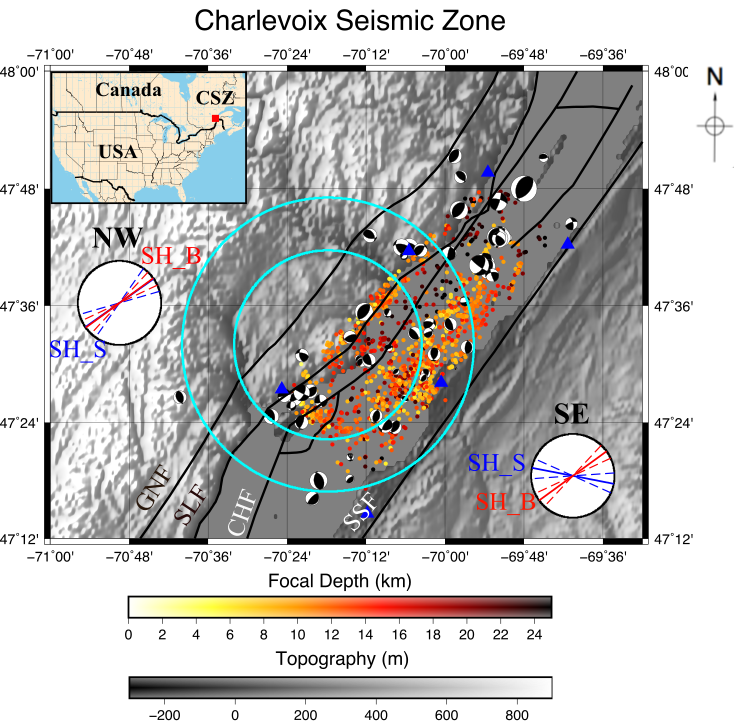
\includegraphics[width=20pc]{Figures/Map_of_CSV_now_w_sta.png} 
\caption{Topography and seismicity of the Charlevoix Seismic Zone (CSZ) showing the location of the impact structure and the seismic stations (blue triangles) (Modified after Fadugba et al., 2019). The locations of the impact structure is represented with the outer cyan circle while the more damaged inner impact structure as the inner cyan circle. Small circles are the relocated epicenters \citep{Powell_2017} and their colors represent the focal depths. The focal mechanisms are for the earthquakes used by \citet{Mazzotti_2010} for the stress inversion. Large circles labeled as NW and SE show orientations of SH$_{\max}$ from the stress inversion of focal mechanism (SH$_S$) and from borehole breakout measurements (SH$_B$) for the earthquake clusters northwest and southeast of the crater center. Solid black lines mark the rift faults known in the region: GNF, Gouffre Northwest Fault; SLF, Saint-Laurent fault; CHF, Charlevoix Fault; and SSF, South Shore Fault \citep{Rondot_1971,lamontagne1999}. The inset shows the location of the CSZ in eastern Canada. Earthquake epicenters are from the National Resources Canada catalog for the years 1988-2011.}
\label{figone}
\end{figure}

Powell and Lamontagne (2017) determined 3D Vp and Vs velocity model of the CSZ, and relocated the earthquakes using the 3D velocity model. Visual estimation of the epicenters in the CSZ shows two major earthquake clusters: the northwestern (NW) and southeastern (SE) clusters. The NW clusters have earthquakes on the Gouffre Northwest fault while the SE clusters comprise of the earthquakes on the Saint-Laurent and Charlevoix faults (Fig. 1). Powell and Lamontagne (2017) also observed circular arcs of seismicity that follow the edge of the impact structure found in 3D tomographic inversions. The presence of damaged crustal crust from the impact crater makes the CSZ an anomalous seismic zone. The presence of the impact crater should decreased the seismicity of the CSZ due to the damaged crustal rocks (Solomon et al., 1987).

Previous studies observed a unique distribution of earthquakes in the CSZ (e.g. Baird et al., 2010) and a stress rotation in the CSZ relative to the regional first-order maximum horizontal stress rotation (Zoback, 2010 & Mazzotti and Townend, 2010). The \textbf{M}4+ earthquakes in the CSZ are concentrated outside the crater, but on the major rift faults, while the small-magnitude earthquakes are located within and beneath the crater region. Despite the high level of seismicity in the CSZ, only a few earthquakes are located on the southwestern part of the crater region (Fig. 1). In addition to the unique distribution of earthquakes in the CSZ, Mazzotti and Townend (2010) observed a significant clockwise rotation in the horizontal stress orientation derived from focal mechanisms relative to the first-order regional stress orientation. Within the CSZ, stress inversion of focal mechanisms of the earthquakes on the NW cluster aligns with the first-order regional stress orientation while that of the southeastern cluster shows a significant clockwise rotation relative to the NW cluster (Mazzotti and Townend, 2010).


%The tectonic history of the CSZ can be broadly divided into four parts. They are: the Grenville orogeny (1100-990 Ma) reflected in amphibolite to granulite metamorphic basement rocks, the breakup of the basement terrains which formed the Iapetus Ocean, Appalachian orogeny formed by the closing of the Iapetus ocean, and the impact crater in the Devonian \citep{Rondot_1971,RONDOT_2000,Baird_2010,}. The basement rocks and Appalachian nappes outcrop in the NW and SE part of the CSZ, respectively, and are separated by Logan’s line (Fig. 2). Logan’s line runs through the center of the crater and along the “north” shore of the St. Lawrence River (Rondot 1994). 

Numerical modeling gives insight into the earthquake distribution and stress rotation in the CSZ (e.g. Baird et al., 2010, Hurd and Zoback 2012, Fadugba et al., 2019). However, these numerical models require a realistic but simplified fault geometry due to the sensitivity of the modeled stress on the fault geometry. Previous work suggests two sets of geometries for the rift faults in the CSZ. One set has a uniform dip of 70$^\circ$SE for all three faults (e.g. Baird et al., 2010), while the second set has 65$^\circ$, 40$^\circ$, and 40$^\circ$SE, from north to south, respectively (Powell and Lamontagne, 2017). Fadugba et al. (2019) used the two fault geometries to model the stress state of the CSZ. Fadugba et al. (2019) observed a partial success of modeled stress concentrations in each two fault geometries in explaining the observed seismicity and stress rotations, which might suggests along-strike variations in the dip angles of the rift faults. Visual estimation of fault planes from over 1300 relocated hypocenters in the CSZ (Powell and Lamontagne, 2017) suggests more complex fault geometry. An important research topic is whether pattern recognition algorithm can be used to determine simplified and realistic fault geometry in the CSZ.

Several work has been done to determine realistic fault planes from the cloud of hypocenters. For example, Ouillon et al. (2008) developed an Optimal Anisotropic Dynamic Clustering (OADC) analysis technique  to delineate fault planes within the aftershocks of the Parkfield earthquake sequences. The OADC method is a pattern recognition method aimed to reconstruct fault networks using the covariance of the spatial distribution of earthquakes from seismic catalogs. Ouillon and Sournette (2011) used the Guassian kernel in a EM method to identify fault planes in intersecting cloud of seismicity, hence intersecting fault planes. Wang et al. (2013b) extended the OADC method to develop Anisotropic Clustering of Location Uncertainty Distributions (ACLUD). The new ACLUD method incorporates some validation steps in order to give the best agreement between the fault planes from a method similar to OADC to the observed focal mechanisms. They also used the uncertainty in the location of each earthquake in the catalog instead of the threshold value assumed in Ouillon et al. (2008). The validation steps proposed by Wang et al. (2013) produce several fault geometries that need the user’s judgment for discrimination.

Based on the assumption that modern seismicity in the CSZ illuminates active faults, I will incorporate focal mechanisms to the Optimal Anisotropic Dynamic Clustering (OADC) algorithm to determine realistic fault planes in the CSZ (Ouillon et al., 2008). I employ a couple of hypotheses in this research. The first hypothesis is that modern seismicity in the CSZ illuminates active faults and can be used to determine the number of the faults, geometries and the interconnectivity of the fault system. The interconnectivity of these faults can be used to predict the maximum magnitude earthquake in the CSZ (Harris et al., 1991; Harris and Day, 1993). If modern earthquakes occur on active faults, then the focal mechanisms of these earthquakes can be used to determine the style of faulting e.g. strike-slip or reverse faulting. In other words, earthquake source mechanisms and seismicity clusters define coherent fault surfaces, hence, the observed slip directions implied by the mechanisms should also be coherent. Based on observed circular arcs of seismicity that follow the edge of the impact structure found in 3D tomographic inversions (Fig. 1, Powell and Lamontagne, 2017), the second hypothesis is that the interface between the crater and the crust can slip and thus can cause earthquakes. High-resolution focal mechanisms of moderate earthquakes (M2 – M4) will then be coupled with the Optimal Anisotropic Dynamic Clustering (OADC) analysis technique to delineate realistic fault geometries. The derived fault geometry from this study will be incorporated in future geodynamic models to determine if the modeled stress result is consistent with the regional stress field and hence provide an explanation for the seismicity of CSZ.



    

 
 
 
 
 
 
 
 
    
\section{Methods}
We use the relocated hypocenters of Powell and Lamontagne (2017) in this study. Powell and Lamontagne (2017) relocated the hypocenters, to an error of less than 1 km, using the 3-D Vp and Vs velocity models determined from a travel time tomography study. Specifically, the hypocenters were relocated with horizontal and vertical errors of 0.15 km and 0.35 km, respectively. Despite the high precision in hypocenter location, the hypocenter shows some unclustered hypocenter probably due to the damaged crustal rocks in the impact structure (Fig. \ref{figone}).

The method used in this study can be broadly divided into two subsections. We first perform declustering analysis on the catalog to remove isolated and diffused earthquakes, in order to highlight the rift faults in the CSZ. Based on the diffuse nature of the background seismicity recorded in the CSZ, the seismicity in the CSZ will be separated into clustered and unclustered events based on the collapsing method (Jones and Stewart, 1997) and cumulative tetrahedra volume (Ouillon and Sornette, 2011). We then apply an Optimal Anisotropic Dynamic Clustering (OADC) algorithm to model realistic fault planes that best fit the hypocenter data. 

In order to avoid spurious fault plane identifications, each cluster of events will be isolated before determining optimal fault planes that minimize the thickness of the cluster. This is necessary because the OADC method will tend to fit the hypocenters with a near-horizontal plane when the depth extent of the earthquakes in a cluster is far less than the areal extent of the cluster. 







The relocated hypocenters of Powell and Lamontagne (2017) have thicker cloud of seismicity about the rift faults, and some earthquakes appear to rim around the impact structure (Fig. 2C). In order to reduce the thickness of the clusters, we applied the collapsing method to account for the location errors in the hypocenters (Jones and Stewart, 1997). 
% For example, the SW cluster clearly shows the two alignments of hypocenters corresponding to two rift faults. The collapsed hypocenters also shows the change in strike of the first rift fault especially near the crater region.
We then applied the cumulative distribution method on the collapsed catalog to remove some of the hypocenters that are isolated. 
%We use a maximum CDF of 0.6 corresponding to about 0.28 km$^{3}$. Figure 4C shows the clustered and unclustered hypocenters in the collapse catalog, while figure 4D shows only the clustered hypocenters. 






\subsection{Declustering analyses}
We used two techniques to decluster the hypocenters: a collapsing method (Jones and Stewart, 1997) and the cumulative distribution of tetrahedra volume method (Ouillon and Sornette, 2011). The collapsing method involves moving each hypocenter within its uncertainty ellipsoid making the collapsed hypocenters within acceptable error in the earthquake location algorithm. The error ellipsoid is constructed with 99.86\% confidence interval (i.e., 4 standard deviations). The idea of the cumulative distribution of tetrahedra volume method is that the volume of a tetrahedral formed by four neighboring hypocenters of unclustered/isolated hypocenters will be higher than those of a clustered hypocenter. Given the small horizontal and vertical errors in the relocation catalog, and the diffuse nature of the seismicity, the cumulative distribution method has little success in separating the clustered hypocenters. To solve this problem, we first applied the collapsing method on the catalog to reduce the variance of the earthquake distribution. and then apply the cumulative distribution method to remove any remaining isolated/unclustered hypocenters.
 
The collapsing method method involves two loops: the first is on each hypocenter while the other loop is on each generation of collapsed hypocenters. We encourage the reader to see Jones and Stewart (1997) for more detailed description and limitations of the method. %in order to clusthe hypocenter relative to thesurrounding hypocenters. 
In summary, the collapsing method involves the following steps: (1) For each earthquake (object earthquake), we find all other earthquakes whose locations lie within the error ellipsoid of the object earthquake using $(\frac{x-x_0}{\sigma_x})^2 + (\frac{y-y_0}{\sigma_y})^2 + (\frac{z-z_0}{\sigma_z})^2 \le s $, where s is related to the confidence interval at the specified degree of freedom. In this study, we use degree of freedom of 3, since the location of the hypocenters are in 3 dimension. (2) Determine the centroid of the earthquakes including the object earthquake, and determine the distance and direction of the centroid to the object earthquake. We then move the object earthquake by a factor of 0.68103 of the distance and in the direction to the calculated centroid (Press et al., 1986). The 0.68103 is necessary for stability (Jones and Stewart, 1997). The location of the object earthquake remains unchanged during this iteration, so the order the hypocenters are processed does not affect the result. 

The outer loop of the collapsing method involves statistical assessment of the movement of the hypocenters, using the following steps: (1) We store the new location of the hypocenters as a new generation of hypocenters. (2) We normalized the movement of object earthquake by corresponding standard deviation, and (3) compare the distribution of the normalized movement with a theoretical chi distribution with degree of freedom of 3. We used chi distribution instead of chi-square distribution because the movement of the hypocenters have been normalized by standard deviation. we then repeat the collapsing method for the next generation of collapsed hypocenters while the locations and sizes of the ellipsoids of uncertainty of the original hypocenter locations remain unchanged. %After collapsing all the hypocenters, there may be some isolated/unclustered hypocenters. %(4) We again applied the cumulative distribution method to remove any isolated hypocenters.

We then apply a cumulative distribution of tetrahedra volume method on the collapsed hypocenters to remove unclustered hypocenters. We compare the distribution of the volumes of the tetrahedra in the collapsed (natural) catalog to the distribution of tetrahedra formed from randomized hypocenters (catalog) in a domain similar to the natural catalog. We generate the randomized catalog by randomizing the x, y and z coordinate of each hypocenter in the collapsed catalog. We randomized the hypocenter in depth as well because of the high number of hypocenters in the upper 15 km thus affecting the distribution of the tetrahedra volume in the randomized catalog. Ouillon and Sornette (2011) did not randomize the depth of the natural catalog.  
%This is similar to the similarity method ($__$). 
%Therefore, it is possible to isolate unclustered events by setting a threshold that is related to the volume of the tetrahedral. 
Following (Ouillon and Sornette, 2011), the cumulative distribution can be summarized as follows. (1) Determine the volume (V) of tetrahedra formed with quadruplets of nearest neighbor events around each hypocenter using equation (\ref{vol_eqn}) for both the collapsed (V) and randomized (V$_0$) catalogs. An apparent challenge occurs when the four nearest neighbor of an isolated hypocenter are clustered. Hence, we used three surrounding hypocenters and the object earthquake to form the tetrahedra. (2) We determine the cumulative distributions of the volumes, i.e., N(V) and $N_0(V_0)$. (3) We determine the volume ($V_0$) of the randomized catalog corresponding to 5\% quantile of the distribution, i.e., probability of 0.05. (4) We then remove all hypocenters in the natural catalog with $V > V_0$, under the assumption that the correlated hypocenters in the collapsed catalog have volumes smaller than the 5\% quantile of the tetrahedra volume distribution in the randomized catalog. %formed by clustered earthquakes have smaller volumes than unclustered earthquakes.

\begin{equation}\label{vol_eqn}
V = \frac{1}{6} \times 
\begin{vmatrix} 
x_{1} &  y_{1} & z_{1} & 1\\ 
x_{2} &  y_{2} & z_{2} & 1\\ 
x_{3} &  y_{3} & z_{3} & 1\\
x_{4} &  y_{4} & z_{4} & 1
\end{vmatrix} 
\end{equation}


 
\subsection{Modified OADC algorithm}
Ouillon et al., (2008) developed the OADC method to determine an optimal number of clusters. OADC method is a generalization of the k-means method using randomly-seeded planes to partition hypocenters into clusters. In this algorithm, we set the minimum ($N_0$) and maximum ($N_{\max}$) number of faults to use in the clustering analysis, in addition to the maximum cluster thickness ($\Delta$) allowed in the algorithm. The value of $\Delta$ should be the same order of magnitude as the maximum radius of uncertainty ellipsoid of the hypocenters. 

The algorithm starts with $N_0$ fault with random positions, orientations, and sizes. The value of $N_0$ is one in this study. In this study, we set the $N_0$, $N_{\max}$ and $\Delta$ to one, five and 0.5 km, respectively. We chose a $N_{\max}$ value of five to account for any along-strike variation of dip angles in the crater region (Fadugba et al., 2019). We partition each hypocenter into different clusters based on its distance to the fault(s). We then determine the covariance matrix (\textbf{C}, equation \ref{covariance_eqn}) of each cluster. The idea of the algorithm is to iteratively determine optimal fault planes that minimize the maximum eigenvalues of the covariance matrix. We perform a principal component analysis on the covariance matrix of each cluster to determine its eigenvectors and eigenvalues. Under the assumption that earthquakes are uniformly distributed over a fault plane, we infer the fault length, width, and thickness from the eigenvalues and the corresponding eigenvectors (Ouillon et al., 2008). This analysis is repeated until the algorithm converges to a fixed geometry. The computation stops when the maximum value of $\lambda_{3}$ in all the clusters is less than the value of $\Delta$. 

\begin{equation}\label{covariance_eqn}
\text{Covariance matrix, \textbf{C}} = \begin{pmatrix} 
\sigma_{x}^2 &  cov(x,y) & cov(x,z)\\ 
cov(x,y) & \sigma_{y}^2 & cov(y,z)\\ 
cov(x,z) & cov(y,z) & \sigma_{z}^2
\end{pmatrix}
\end{equation}

According to Ouillon et al., 2008, we attribute the largest eigenvalues ($\lambda_1$) to the length of the cluster, and the azimuth of the corresponding eigenvector to represent the strike of the fault. In addition, we use the intermediate ($\lambda_2$) and smallest ($\lambda_3$) eigenvalues to infer the width and thickness of the fault planes, respectively. The barycenter of each cluster (e.g., $x_b$ = mean(x)) coincides with the center of the fault. Based on a statistical method, Ouillon et al., (2008) estimated the length (L) and width (W) of the fault plane using  $\lambda_{1}\sqrt{12}$ and $\lambda_{2}\sqrt{12}$, respectively. The value of $\lambda_{3}$ gives information on the thickness of the cluster. The strikes and dips of the fault planes are determined from the eigenvector of the minimum eigenvalue ($\lambda_{3}$) of each cluster.

However, if the maximum $\lambda_{3}$ in the stable fault geometry is greater than $\Delta$, the fault in thickest cluster is replaced by at least two new faults with random locations and orientations within the cluster. The lengths of the new faults are one-half that of the original thick fault. We perform the splitting process several times (20 times in this study) to determine the random fault geometry that gives the least maximum $\lambda_3$ at the resulting fixed geometry. The number of fault increases by one, and the covariance matrix analysis is repeated. The simulation stops when the value of $\lambda_3$ is less than the value of $\Delta$, or the $N_{\max}$ is reached.

In this study, we incorporate the focal mechanisms into the OADC algorithm to split the 'thick' cluster instead of using a randomly-seeded planes. We use any available high-quality focal mechanisms of earthquakes that are within or at a distance of 1 km to the thick cluster. We assign the first two dominant strike direction of the focal mechanisms and the average of their corresponding dips to two faults. %The orientation of the second is chosen at random among any other strike distribution and their corresponding dips 
Wang et al., 2013 also incorporate focal mechanisms to OADC in their the ACLUD method, but as a validation step after determining several results from OADC-type algorithm. 


The idea is to plot the nodal plane normal vectors for earthquakes with high-quality source mechanisms and use the dominant orientations to specify the planes in the OADC method rather than using randomly-seeded planes. 

%The dot products of the nodal plane normal vectors of each earthquake and that of the dominant planes will then be used as a clustering mechanism in addition to the standard clustering method of OADC for earthquakes with no focal mechanisms.

%In order to avoid near horizontal fault planes, we set the minimum dip angle allowed in the algorithm. So, we rotated all the fault planes with dip angles below the minimum dip angle by 90$^\circ$ along its strike within the iteration.

% A 3D joint relocation of the earthquakes in the CSZ using recent 3D tomography results will be used to determine the dependence of the method on the location accuracy.


We assigned the modal strike and penultenate strike angles to the two new faults, and use the average of all the dip angles in the focal mechanisms corresponding to the chosen strike angles. 







\section{Results}

\subsection{Declustering analyses}
We determine the volume of the tetrahedra defined by closest hypocenters for each 1329 earthquakes in the CSZ (Fig. domA, Powell and Lamontagne, 2017). The volumes of the tetrahedra ranges from 9.45 $\times 10^{-5}$ to about 31.61 km$^{3}$. We also generated a randomized catalog within a  65- x 65- km domain size similar to the seismic zone (Fig. domB). The tetrahedra volume in the randomized catalog ranges from 0.003422 to 26.74 km$^{3}$.

\begin{figure}[ht]
\centering
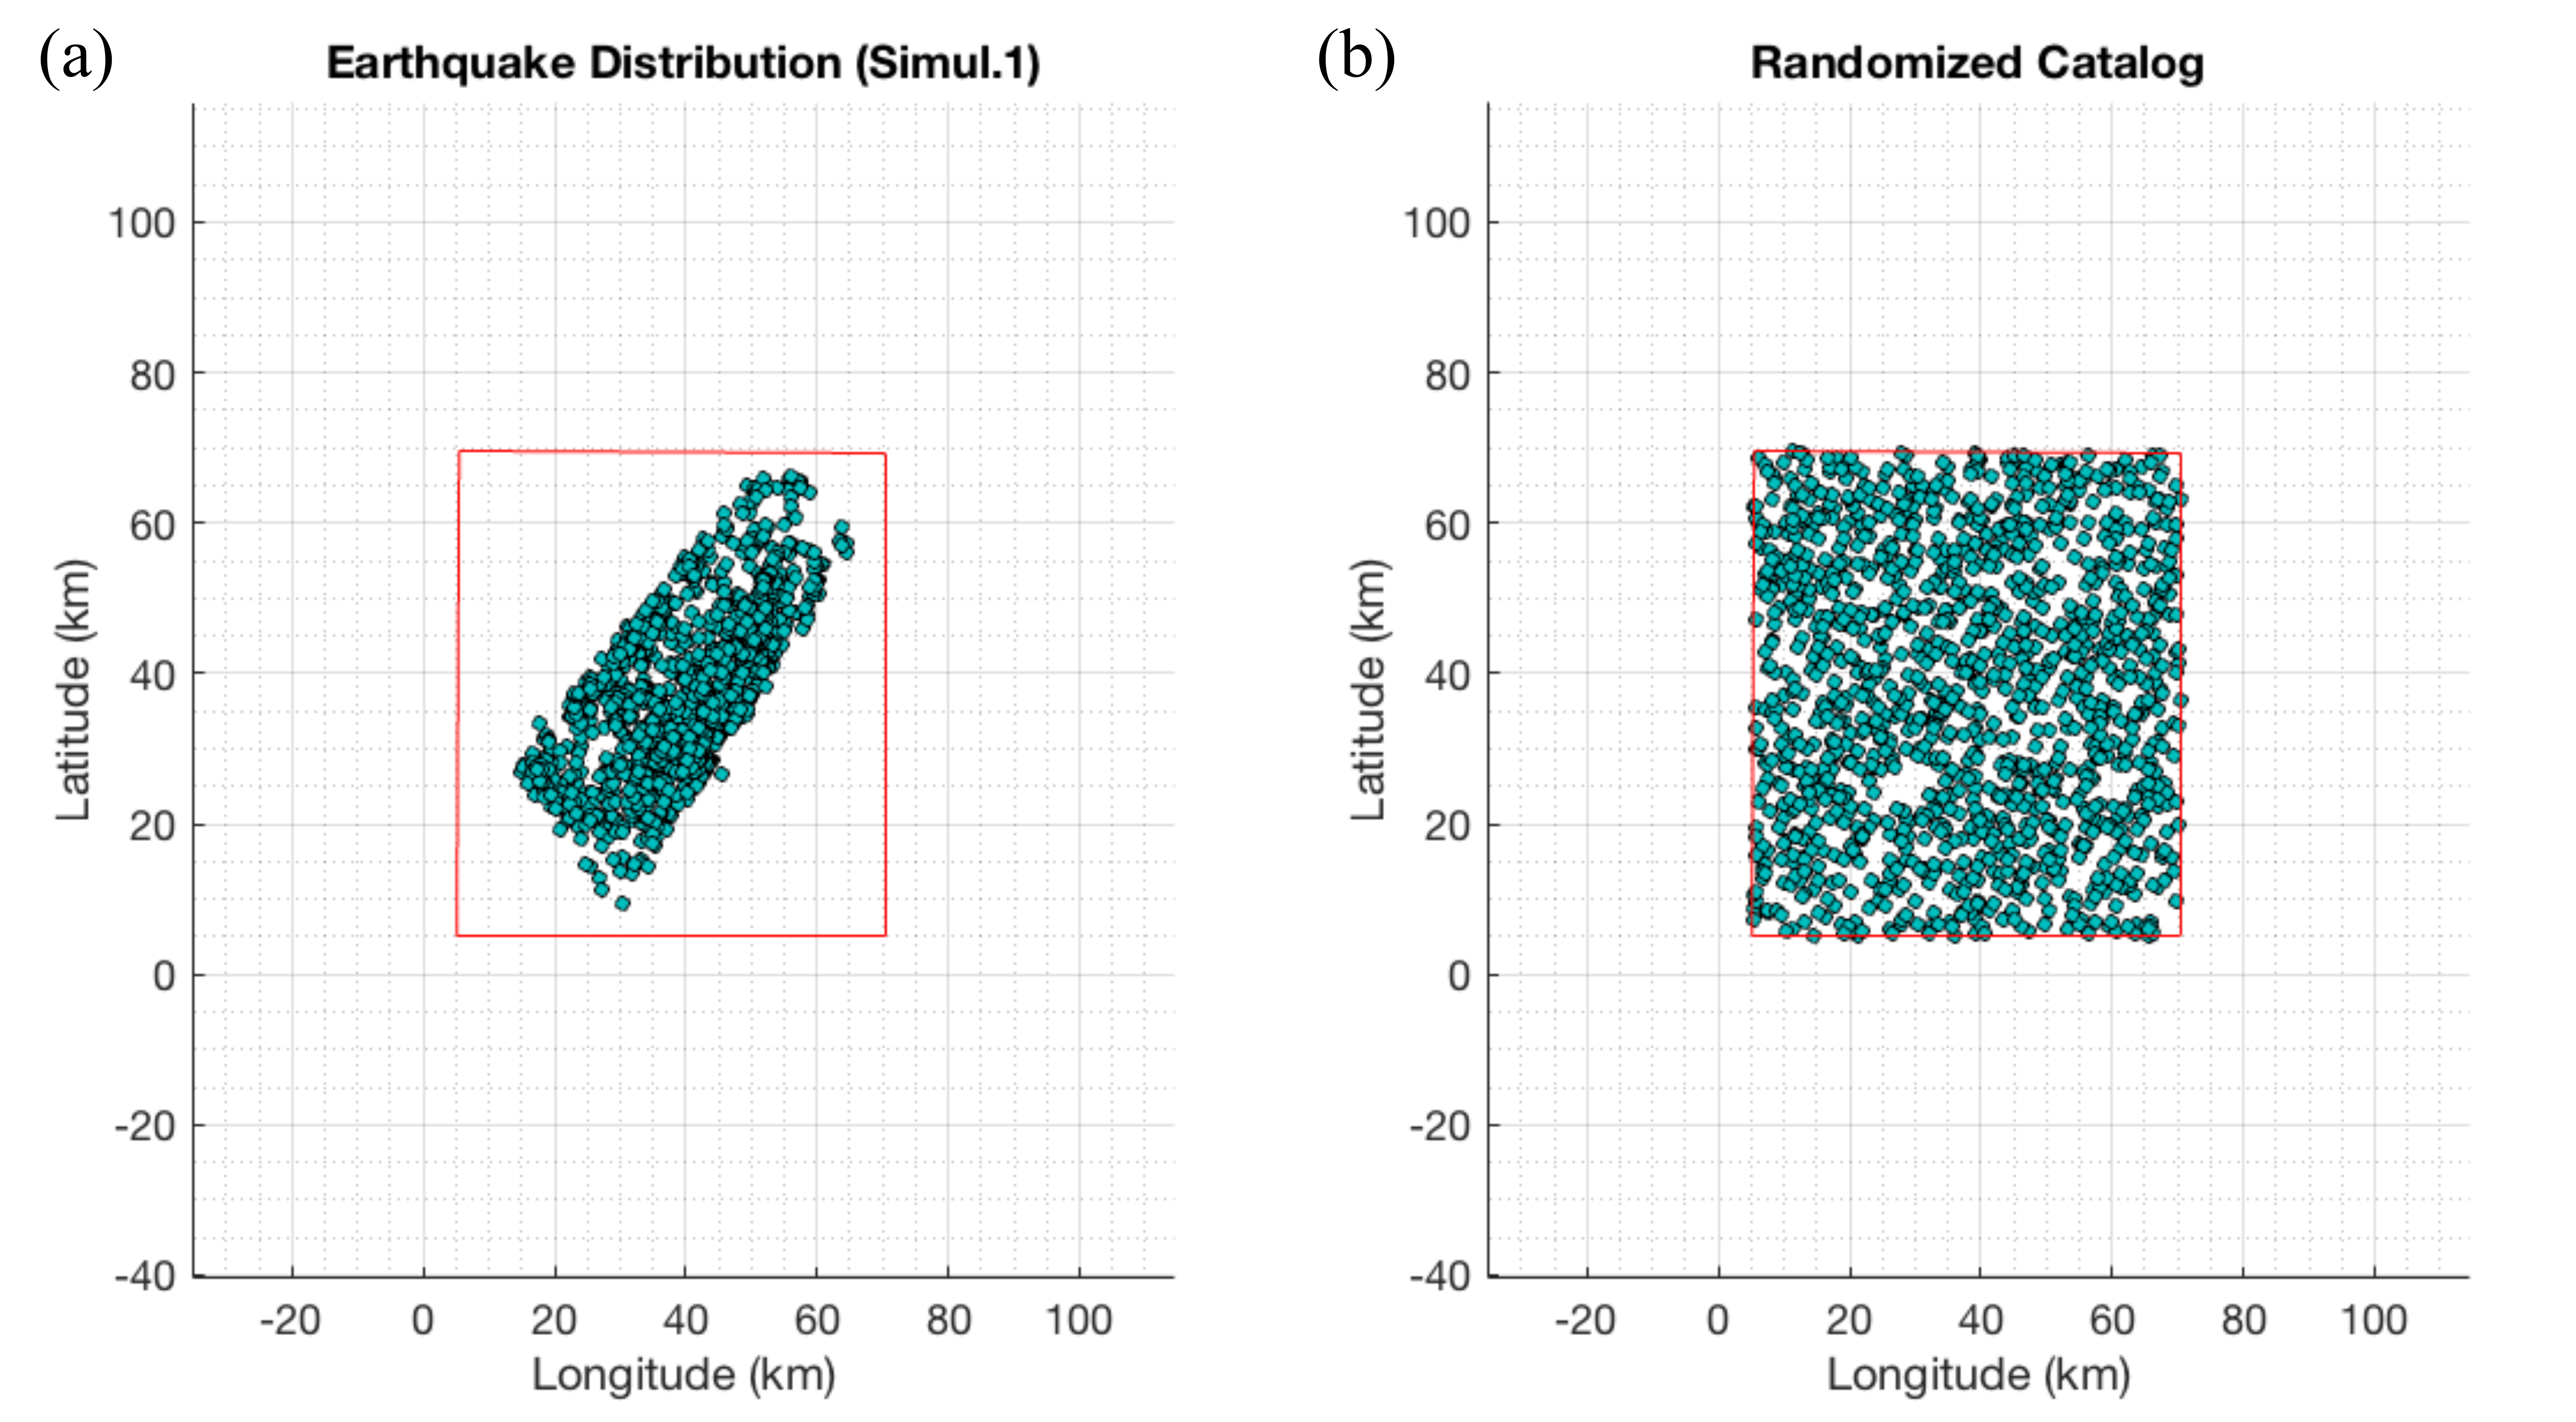
\includegraphics[width=25pc]{Figures/domain_cum_only.png}
\caption{Domain of the seismic zone to generate randomized catalog.}
\label{figfive}
\end{figure}

We determine the cumulative distribution function (CDF) of the tetrahedra volume of both catalogs (Fig. cdf). The volume at 5 percent probability (V05) is 0.08389 km$^{3}$ and the probability at target volume (N(V05)) = 0.5774 (Fig. cdf). This method removes 562 diffused/unclustered earthquakes (42.29\% of the original catalog). Figure \unclusteredA shows the superposition of clustered and unclustered hypocenters while figure \unclusteredA shows only the diffuse/unclustered hypocenters. The unclustered earthquakes show no significant alignment which may depict concentration of hypocenters on main rift faults. 

\begin{figure}[ht]
\centering
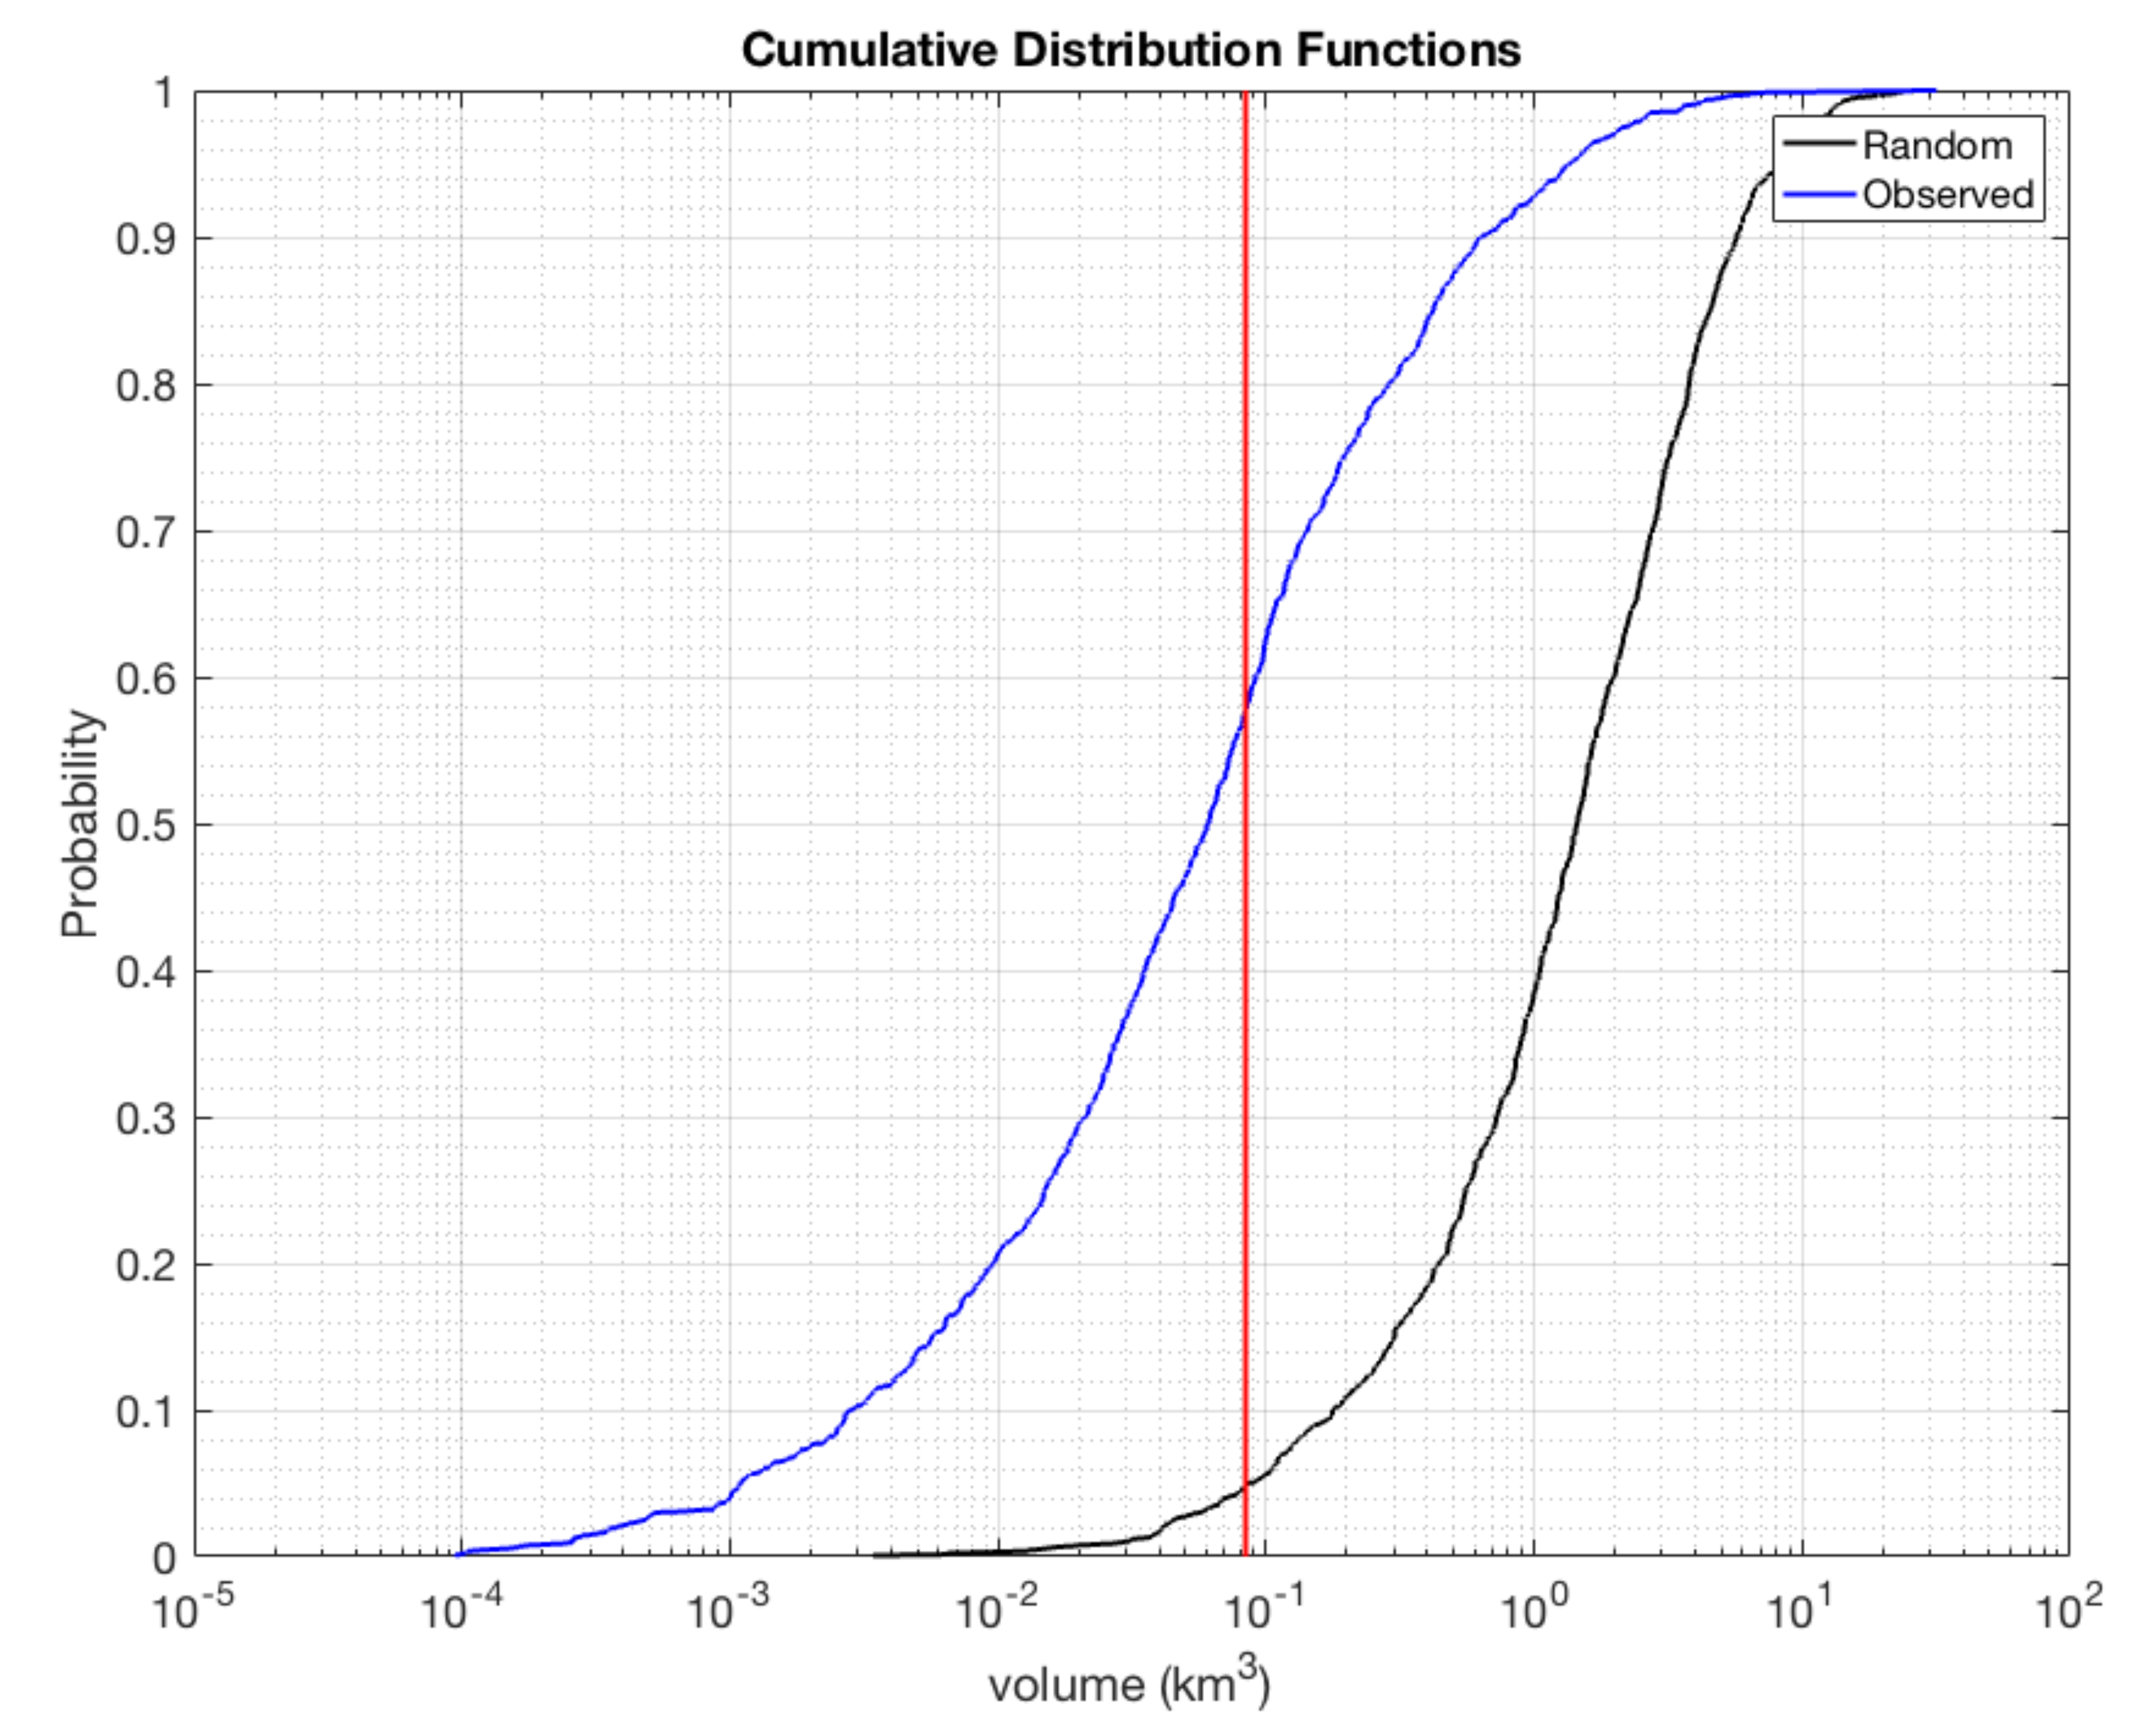
\includegraphics[width=25pc]{Figures/cdf_cum_only.png}
\caption{cumulative distribution curve for hypocenters of the earthquakes of the CSZ.}
\label{figfive}
\end{figure}

\begin{figure}[ht]
\centering
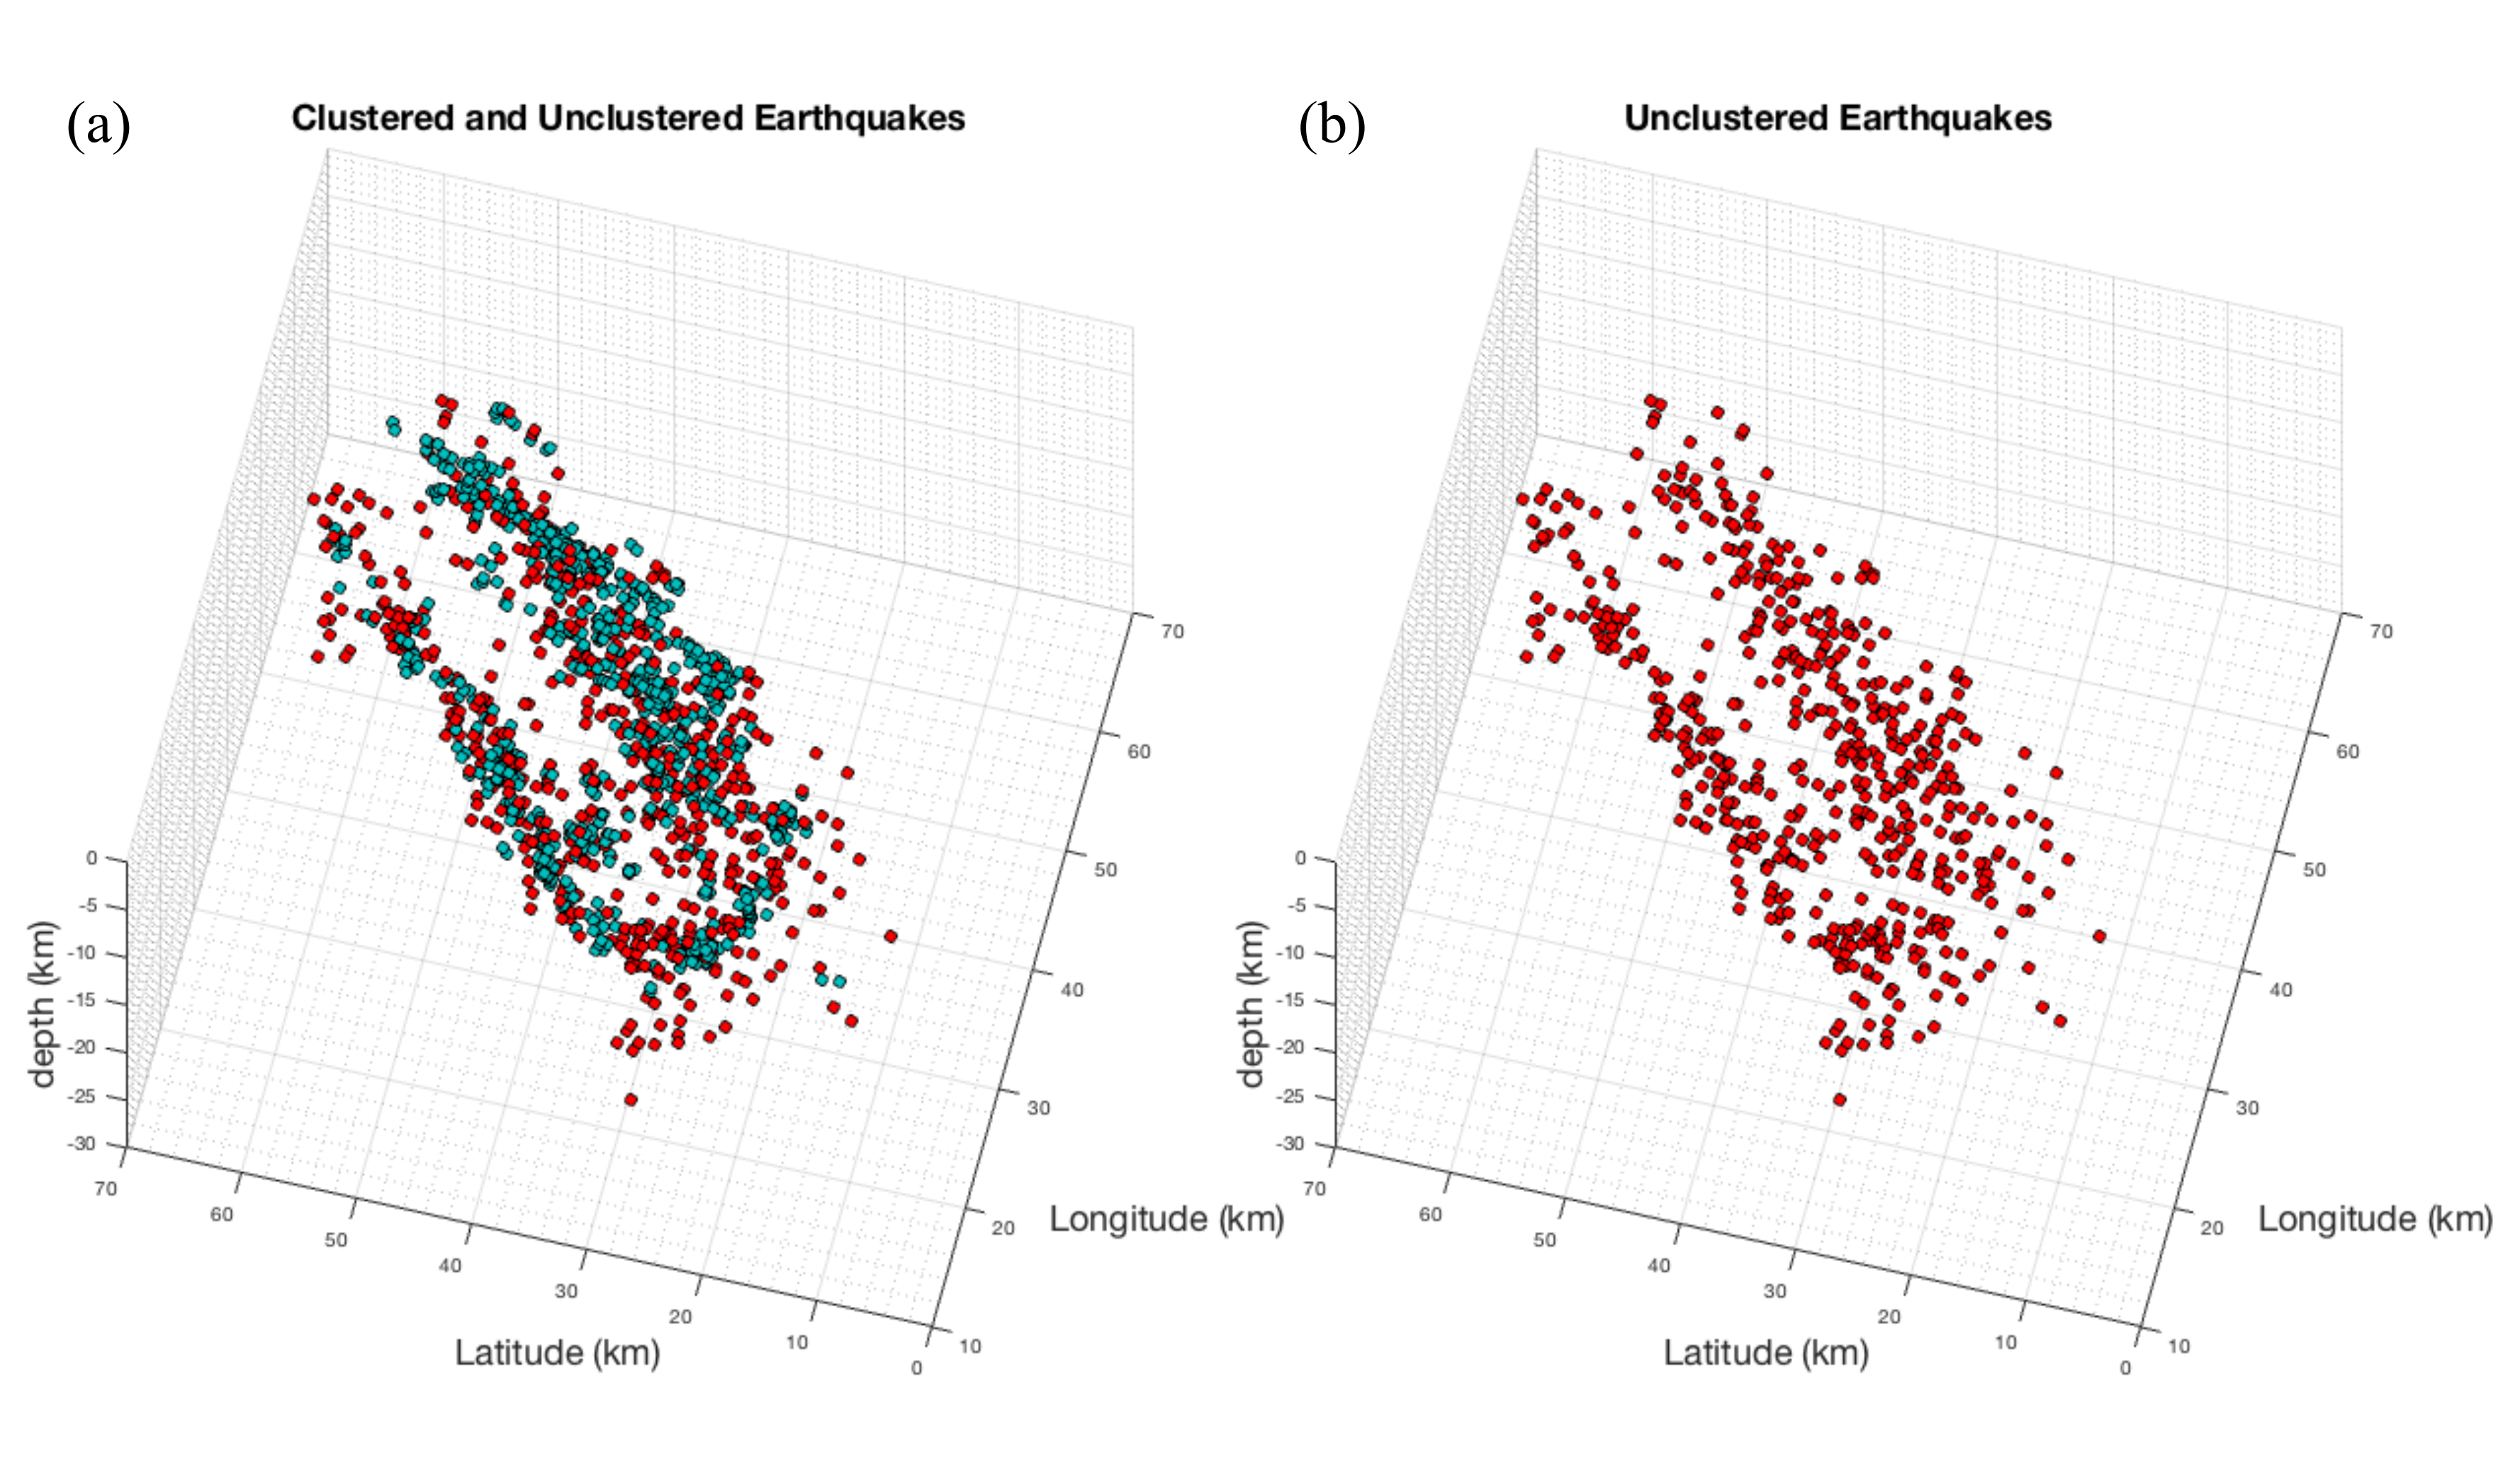
\includegraphics[width=25pc]{Figures/unclustered_cum_only_results.png}
\caption{Unclustered hypocenters.}
\label{figthree}
\end{figure}

%The clustered and unclustered hypocenters give interesting incite to the seismicity of the CSZ. For example, 
The clustered hypocenters occur on identifiable alignment related to the main rift faults in the CSZ (Fig \cum_results b) compared to the full relocated hypocenters of Powell and Lamontagne (2017) (Fig \cum_results a). The clustered earthquakes also reveal some hypocenters in the related to the impact structure. Figures \cum_results c and d are the same as \cum_results a and b, respectively, but using different viewpoints that emphasizes the result of declustering algorithm.

\begin{figure}[ht]
\centering
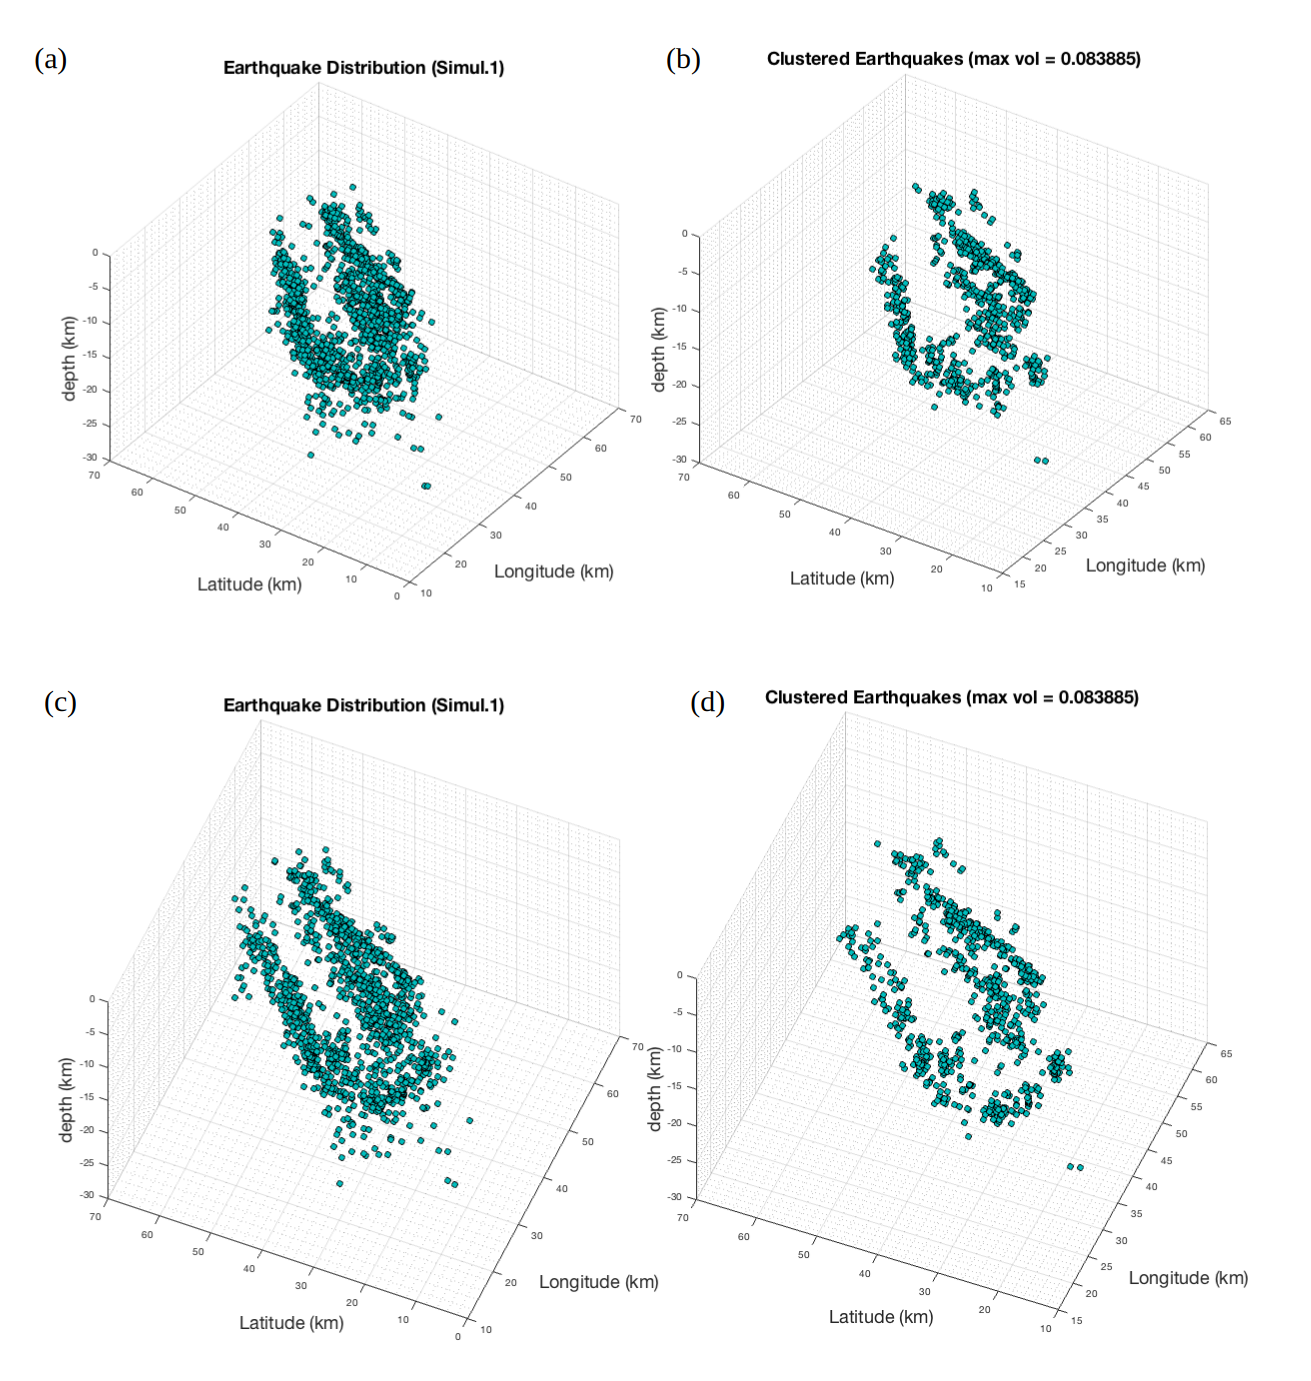
\includegraphics[width=25pc]{Figures/cum_only_main_results.png}
\caption{Clustering of earthquakes in CSZ using modified cumulative distribution method.}
\label{figtwo}
\end{figure}
  
 
\subsection{Fault plane geometry of the CSZ}
Fig 6A is an intermediate result showing the best-fit plane using one fault. The plane is gently dipping to the southwest. This one fault is the thickest fault, and was splitted into two faults with one-half its original length. To generaate the two starting faults, we use focal-mechanism seeded planes rather than the randomly-seeded planes in the original OADC algorithm. We determine the strike distribution of available focal mechanisms within the thick cluster using 20 number of bins (Fig. 6B). The strike angles of the two faults are 28$^\circ$ and 10.8$^\circ$, respectively, while their corresponding average dip angles are 55$^\circ$ and 62$^\circ$, respectively. We generated the new fault planes, with their centers placed them at random positions within the cluster to determine the configuration with the lowest $\lambda_3$ value. We repeated the random position of the new faults 6 times in this study, to determine the positions with the best stable fault geometries assumed to be the one with the lowest $\lambda_3$ value. Figures 6 c and d show two examples of random positions of the focal-mechanism-seeded fault planes. Figure 6 e shows the intermediate stable fault plane geometries using two faults. The two faults captures the NW and SE earthquake clusters, but with a larger minimum $\lambda_3$ values compared to the input threshold (0.001 km).

We further determine the cluster with the largest $\lambda_3$ value, and split the cluster using the above procedure. the OADC algorithm was fitted one fault to the NW and another one to the SE clusters, and also fitted the earthquakes beneath the crater with a near-horizontal fault (Fig. 7a) similar to the two-fault model in figure 6e. The near-horizontal fault in the 3-fault model was corrected when the number of fault increases to 4 (fig 7B). The intermediate fault model now distinguished the two rift faults in the SE cluster, and the NW cluster with two faults of different strike and dip angles. 

%We got geologically feasible fault planes when the number of faults is 5 (Fig. 8). The OADC fitted the SE cluster with two fault planes with dip angles of 46.8$^\circ$ and 47.2$^\circ$, respectively with a maximum $\lambda_3$ value of 1.6242. The NW cluster was fitted with a steeper faults with a dip of 58.5$^\circ$. Within the impact structure region in the NW cluster, OADC fitted two more faults with shallower dips of 48.6$^\circ$ and 34.8$^\circ$ in the direction of the impact structure. Table 1 shows the summary of fault geometry from the OADC algorithm. 

%The OADC produced another geologically feasible fault geometry with a smaller $\lambda_3$ value of 1.5293, but with a higher dip angles for the faults in the SE cluster. The two faults dip at 57.9$^\circ$ and 48.7$^\circ$, respectively instead of the 46.8$^\circ$ and 47.2$^\circ$ in the previous model. The NW fault also dips at an higher angle of 62.9$^\circ$ compared to the 58.5$^\circ$ in the previous model. 

e got geologically feasible fault planes when the number of faults is 5 (Fig. 8). The OADC fitted the SE cluster with two fault planes with dip angles of 46.8$^\circ$ and 47.2$^\circ$, respectively with a maximum $\lambda_3$ value of 1.5293. The NW cluster was fitted with a steeper faults with a dip of 62.9$^\circ$. Within the impact structure region in the NW cluster, OADC fitted two more faults with shallower dips of 48.6$^\circ$ and 34.8$^\circ$ in the direction of the impact structure. Table 1 shows the summary of fault geometry from the OADC algorithm. 

The OADC produced another geologically feasible fault geometry with a slightly higher $\lambda_3$ value of 1.6242, but with a higher dip angles for the faults in the SE cluster. The two faults dip at 46.8$^\circ$ and 47.2$^\circ$, respectively instead of the 57.9$^\circ$ and 48.7$^\circ$ in the previous model. The NW fault also dips at an higher angle of 58.5$^\circ$ compared to the 62.9$^\circ$ in the previous model. 


    \begin{table}
    \caption{Fault geometry of the CSZ using OADC method.}
    \centering
    \begin{tabular}{ccccccccc}
    \hline
    Fault No &   & \multicolumn{2}{c}{Fault Model 1$^{a}$} & &  \multicolumn{2}{c}{Fault Model 2$^{a}$} &   &Possible mapped fault \\
    & & Strike & Dip  & & Strike & Dip & & \\
    \hline
    1 & &24.3$^\circ$ & 48.7$^\circ$ &  &     24.5$^\circ$ & 47.3$^\circ$& &Charlevoix fault \\
    2 & &5.8$^\circ$ & 22.5$^\circ$ & 	&	8.6$^\circ$ & 34.3$^\circ$& &Crater boundary  \\
    3 & &30.5$^\circ$ & 57.9$^\circ$ & 	&	32.8$^\circ$ & 46.8$^\circ$&  &Saint-Laurent fault\\
    4 & &24.1$^\circ$ & 50.2$^\circ$ & 	&	27.8$^\circ$ & 48.6$^\circ$&  &Crater boundary \\
    5 & &33.1$^\circ$ & 62.9$^\circ$ & 	&	36.3$^\circ$ & 58.5$^\circ$&  &Gouffre Northwest fault\\
    \hline
    \multicolumn{9}{l}{$^{a}$ $\lambda_{3,max}$ for fault models 1 and 2 are 1.53 and 1.62, respectively.}
    %\multicolumn{3}{l}{$^{1}$\citet{lamontagne1999}. \text{syntax: vel\_model = [vp vs rho depth layer\_no]}}
    \end{tabular}
    \label{tableone}
    \end{table}




\begin{figure}[ht]
\centering
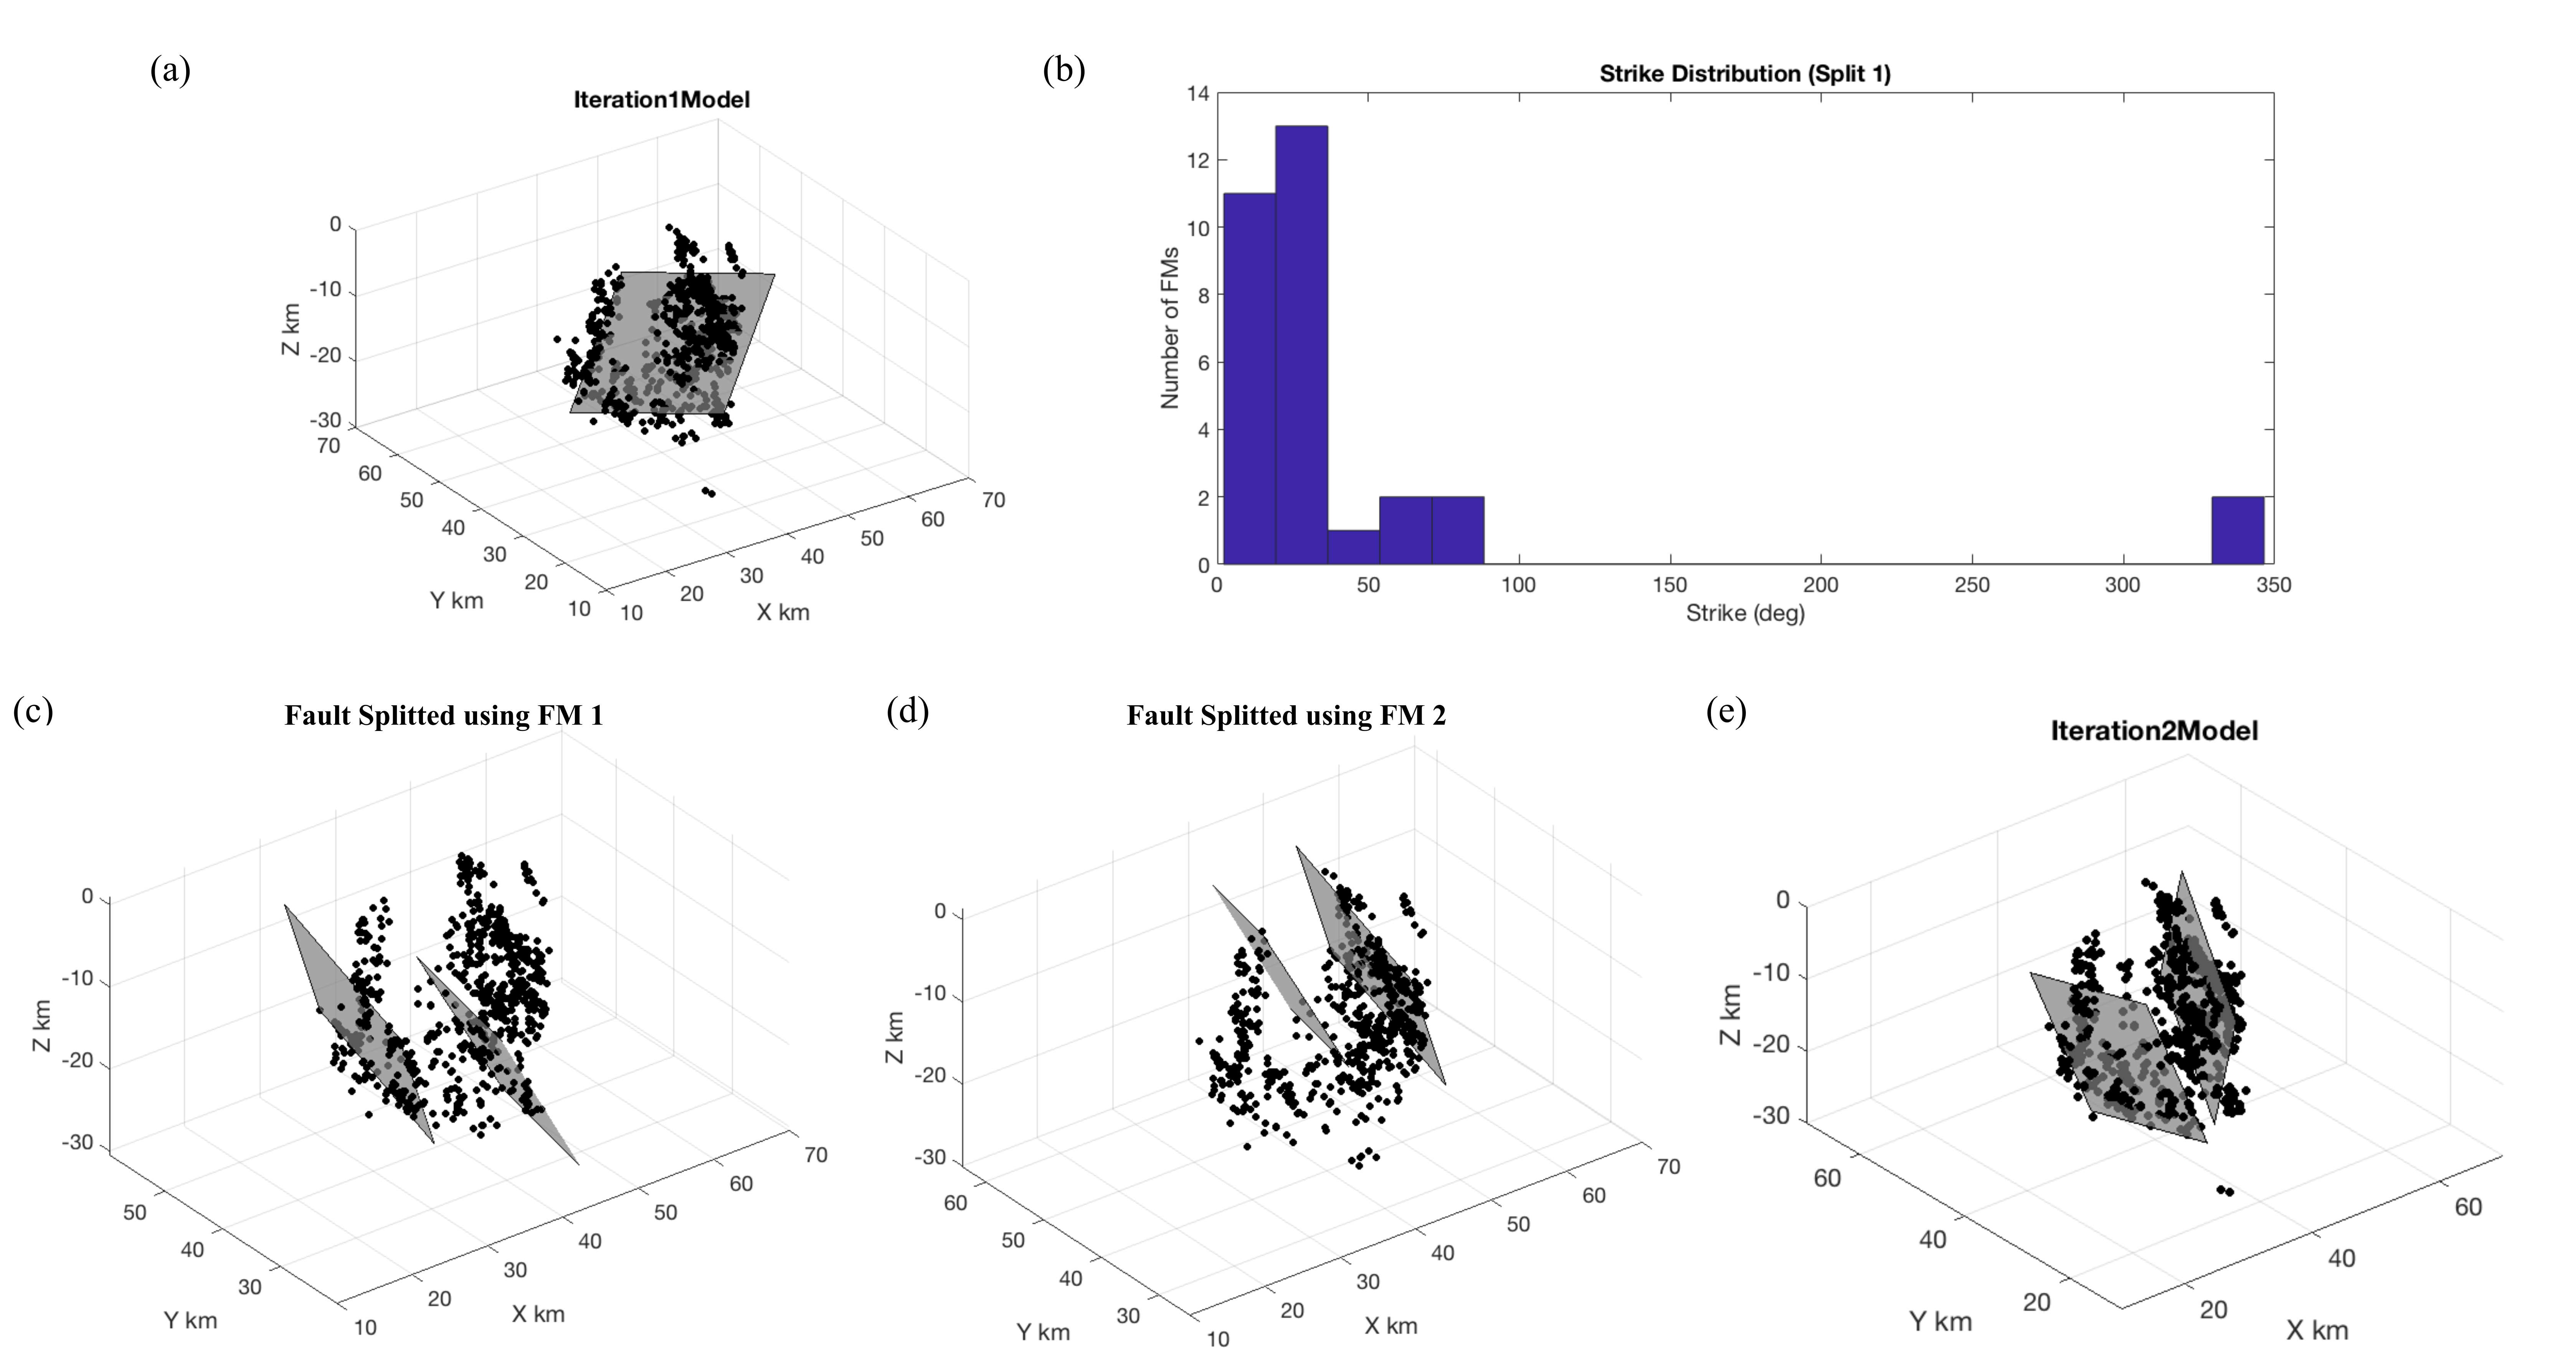
\includegraphics[width=25pc]{Figures/OADC_fig_1.png}
\caption{Intermediate fault models of OADC method on the clustered earthquakes.}
\label{figsix}
\end{figure}

\begin{figure}[ht]
\centering
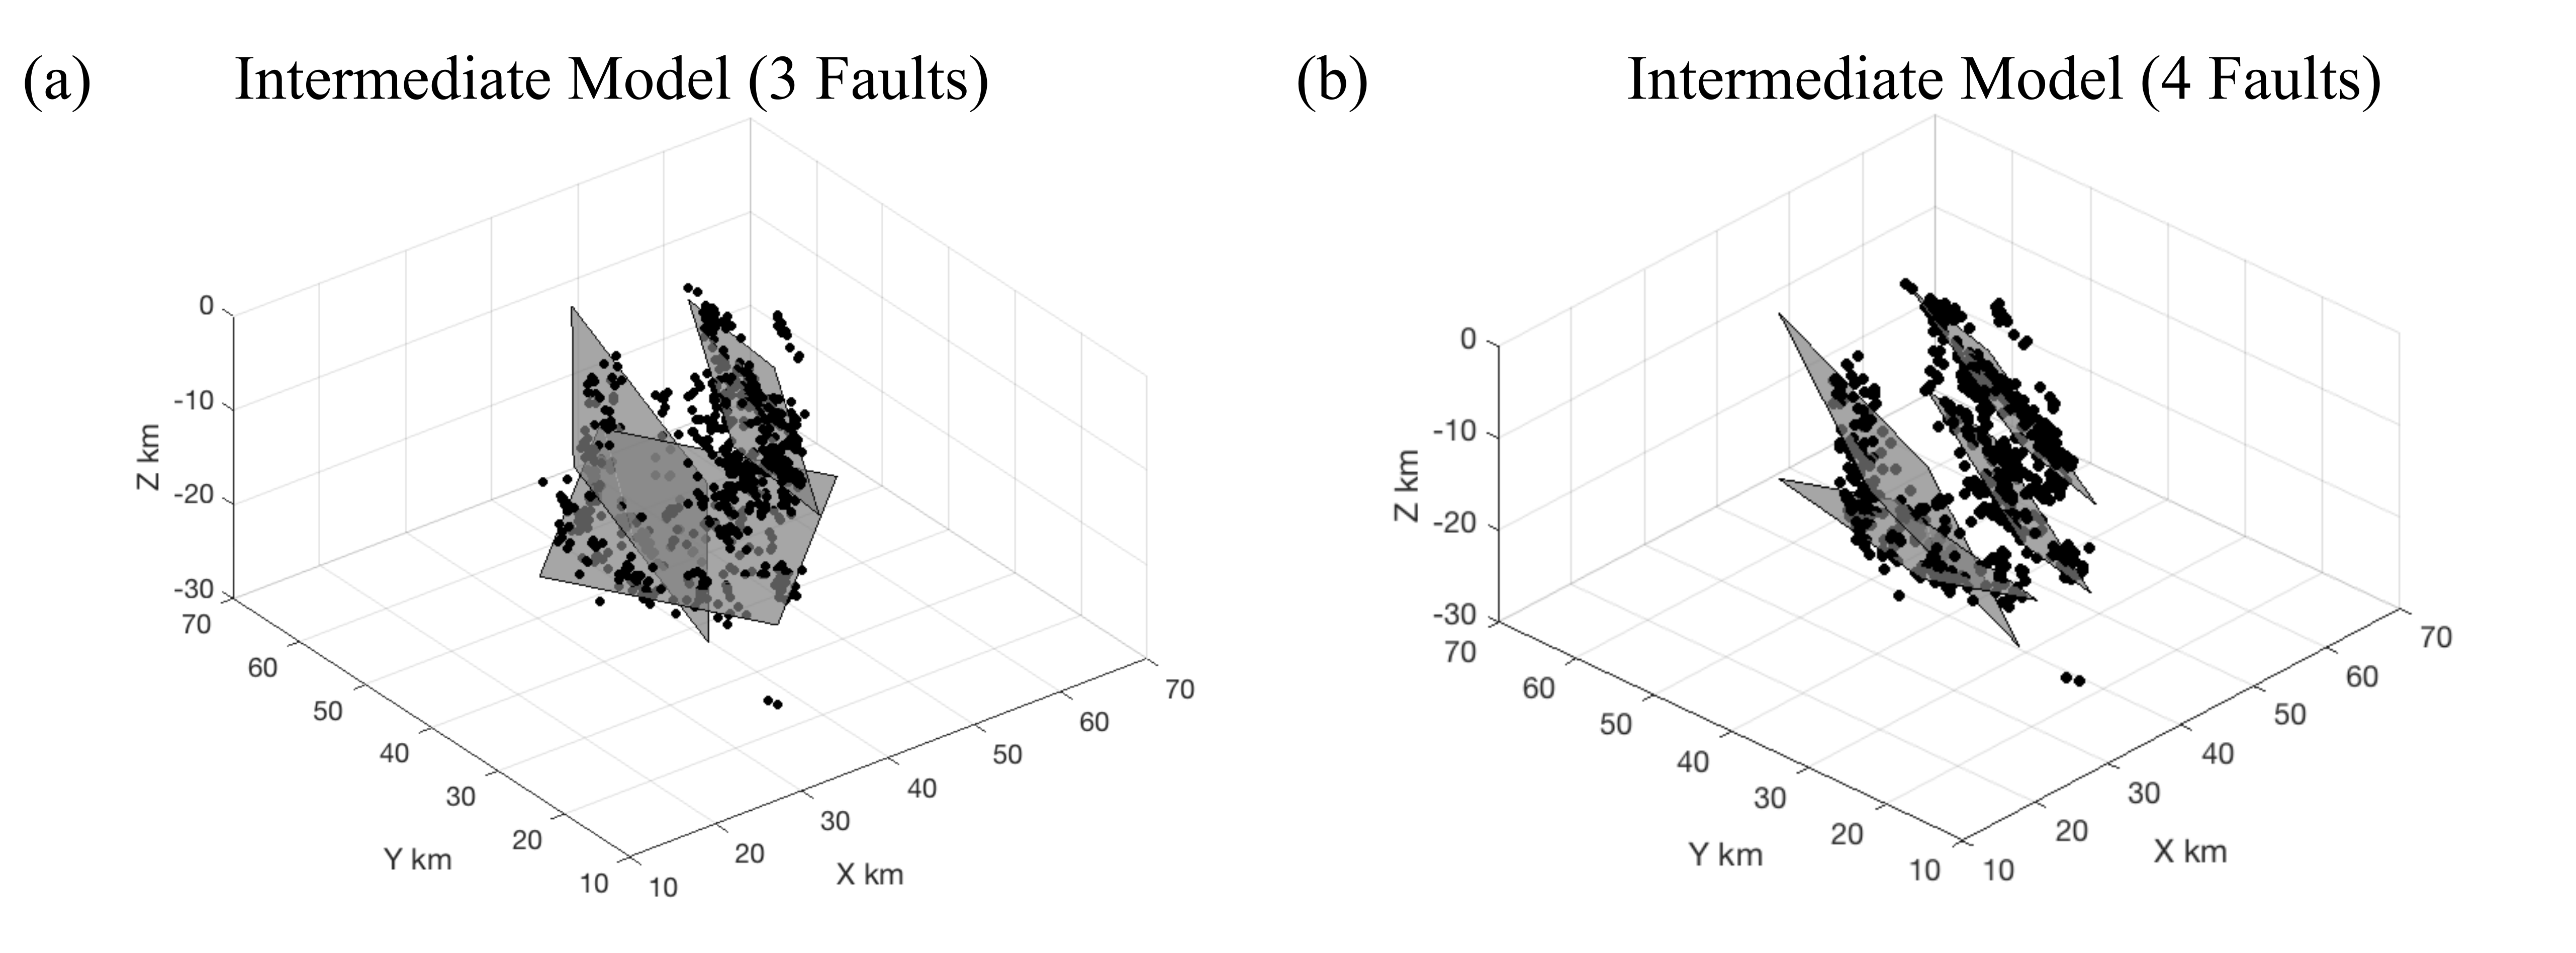
\includegraphics[width=25pc]{Figures/OADC_fig_2.png}
\caption{Intermediate fault models of OADC method on the clustered earthquakes.}
\label{figsix}
\end{figure}


\begin{figure}[ht]
\centering
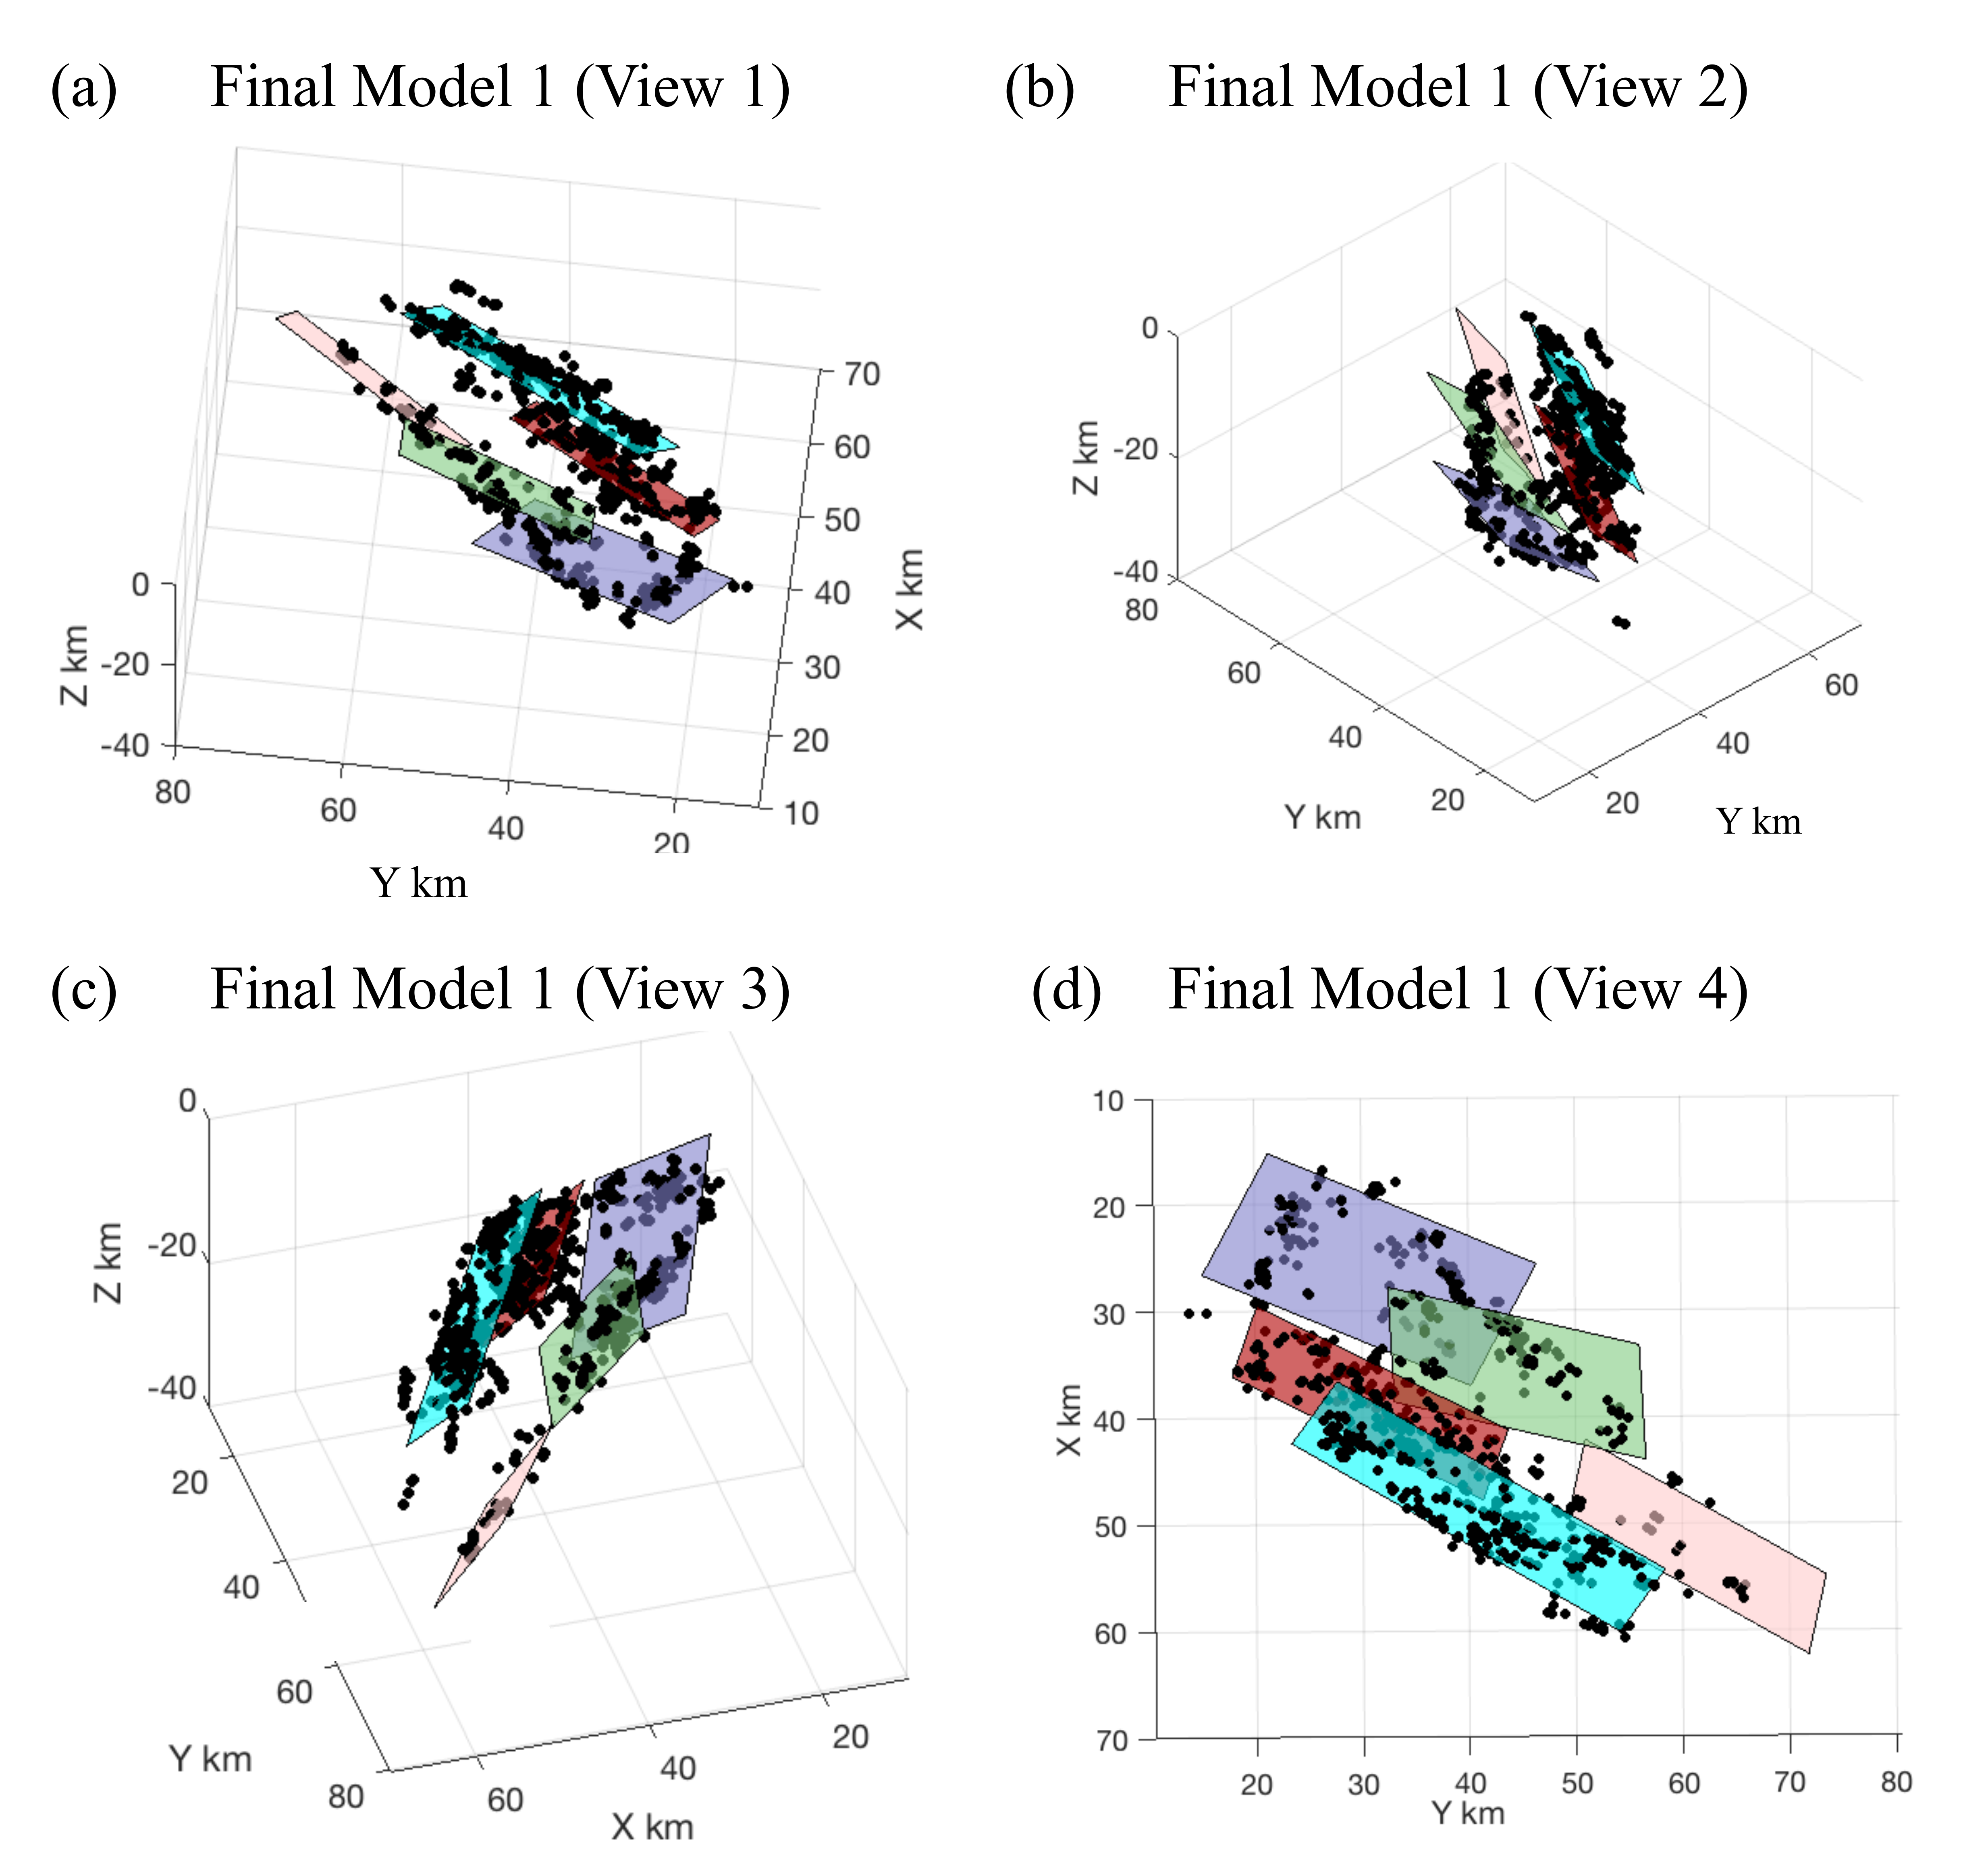
\includegraphics[width=25pc]{Figures/OADC_fig_final1.png}
\caption{Final fault models of OADC method on the clustered earthquakes.}
\label{figsix}
\end{figure}

\begin{figure}[ht]
\centering
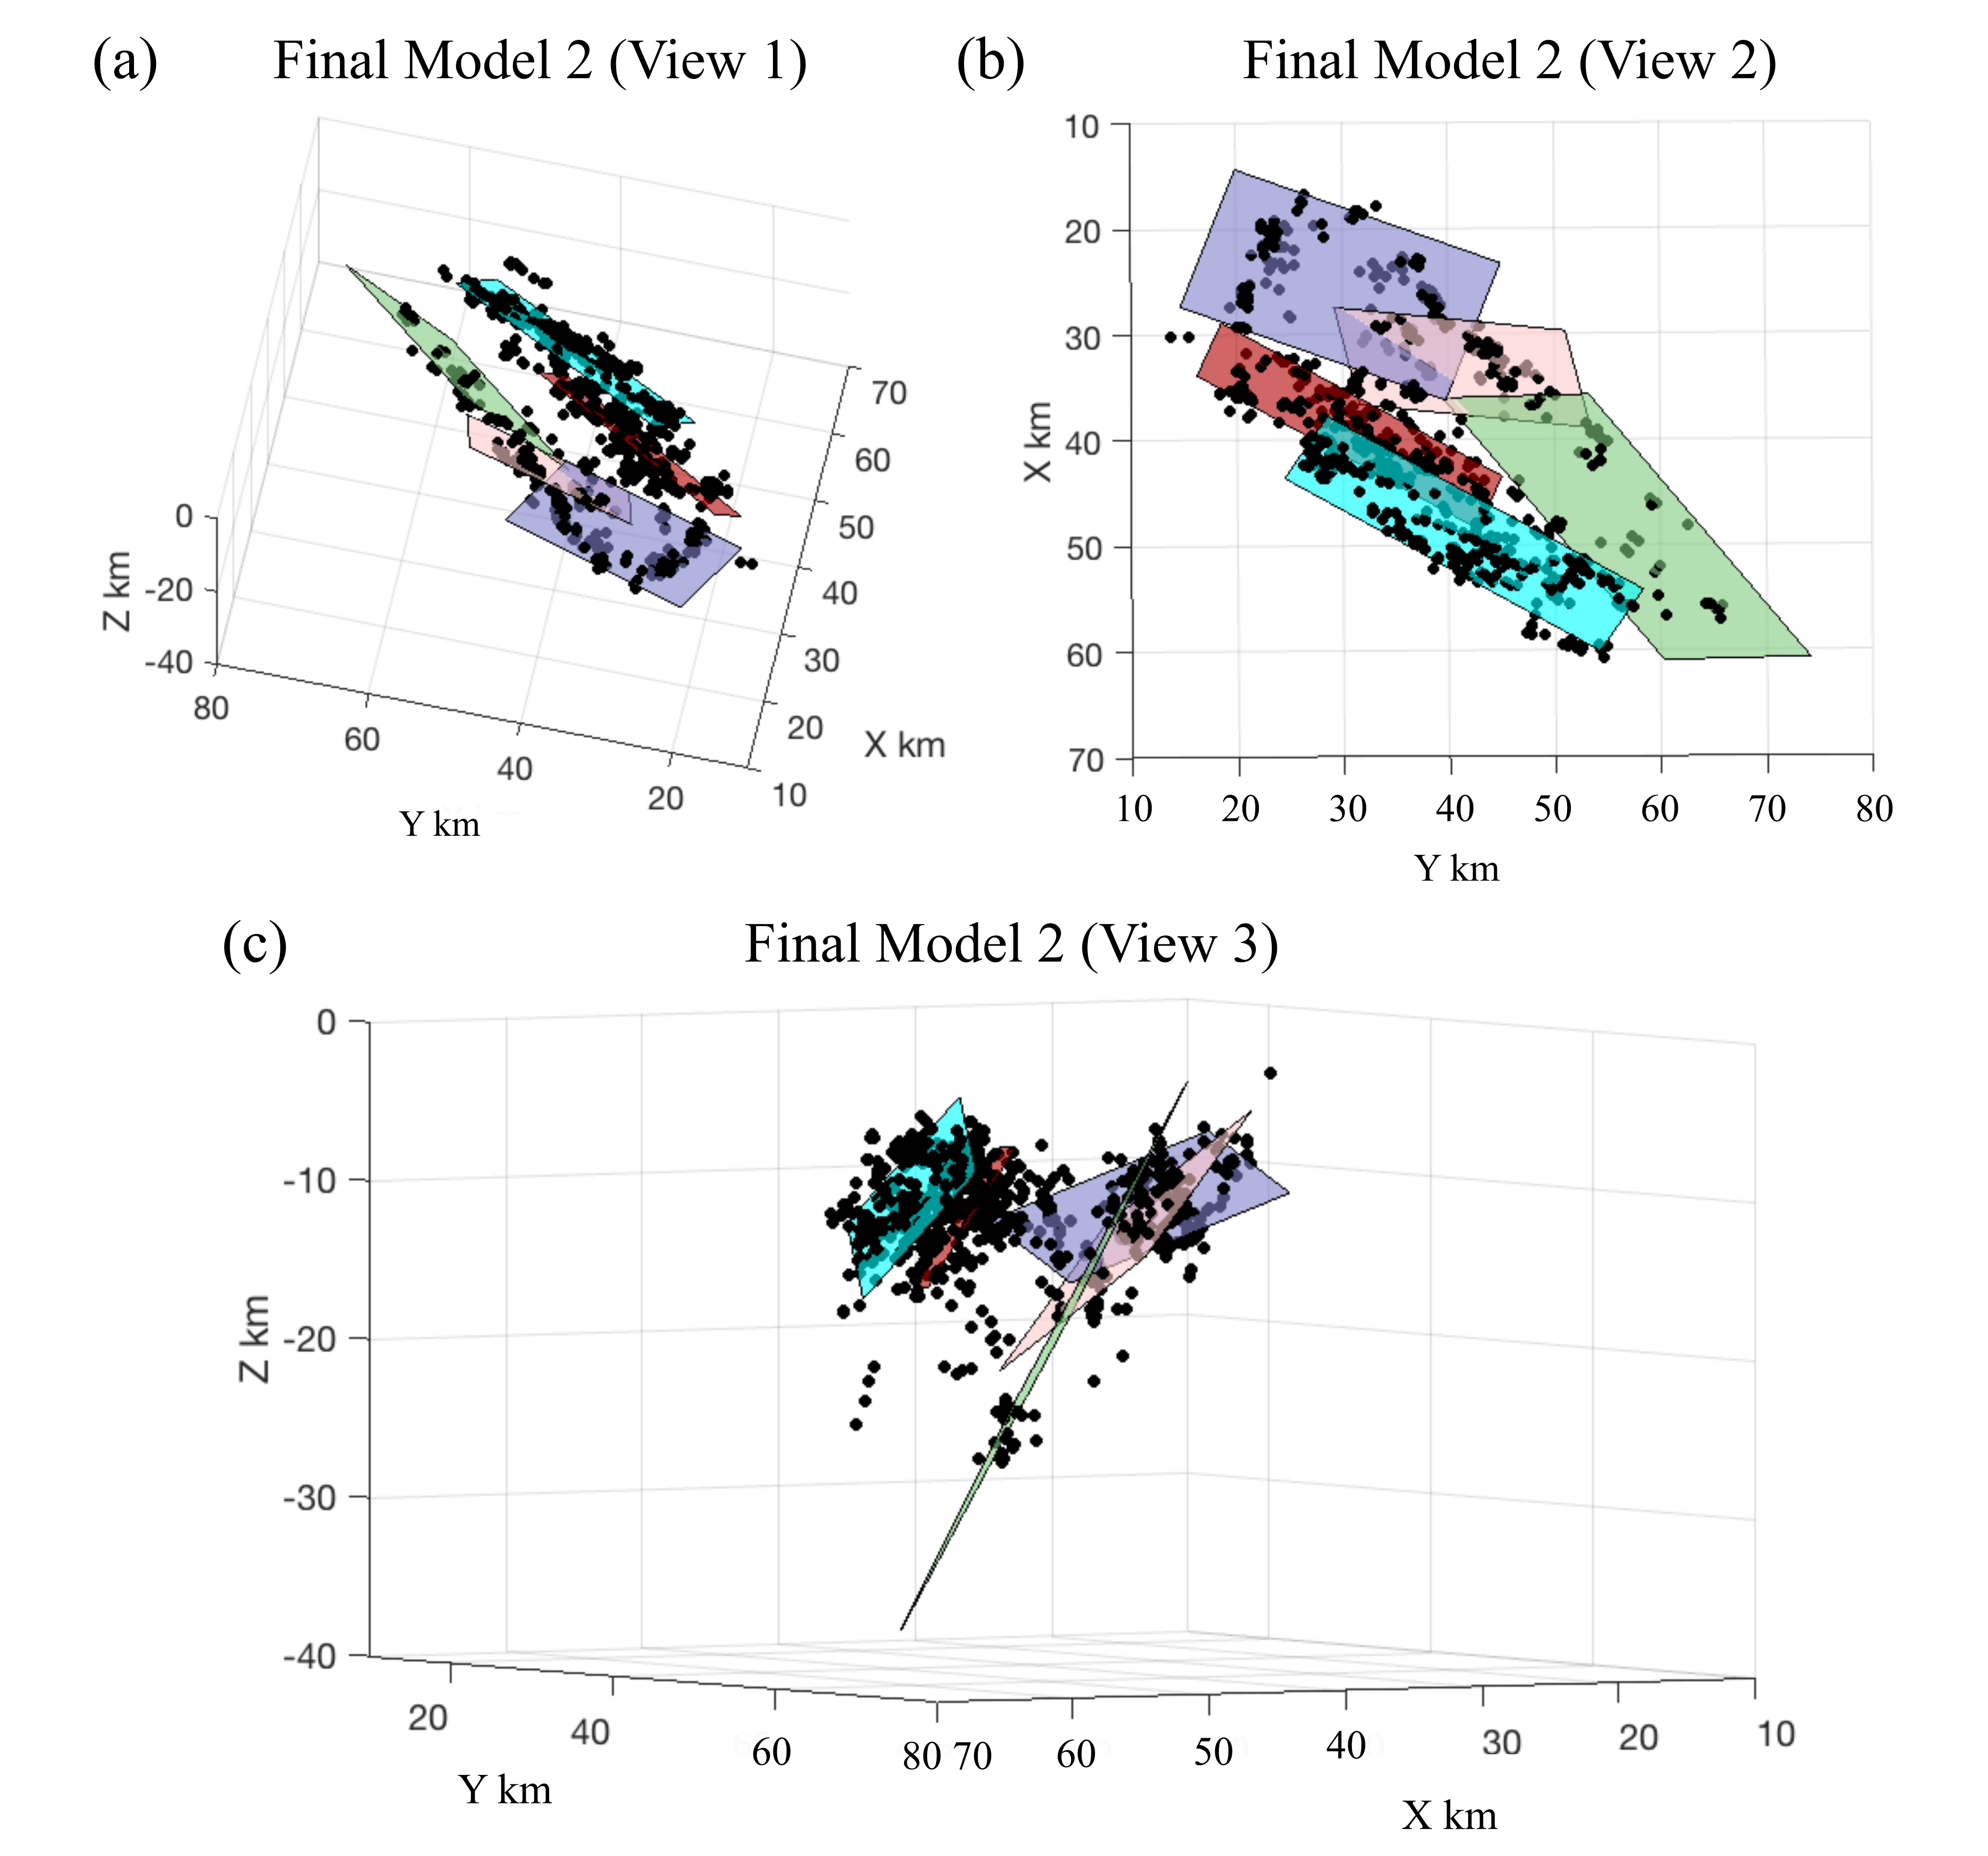
\includegraphics[width=25pc]{Figures/OADC_fig_final2.png}
\caption{Final fault models of OADC method on the clustered earthquakes.}
\label{figsix}
\end{figure}


\begin{figure}[ht]
\centering
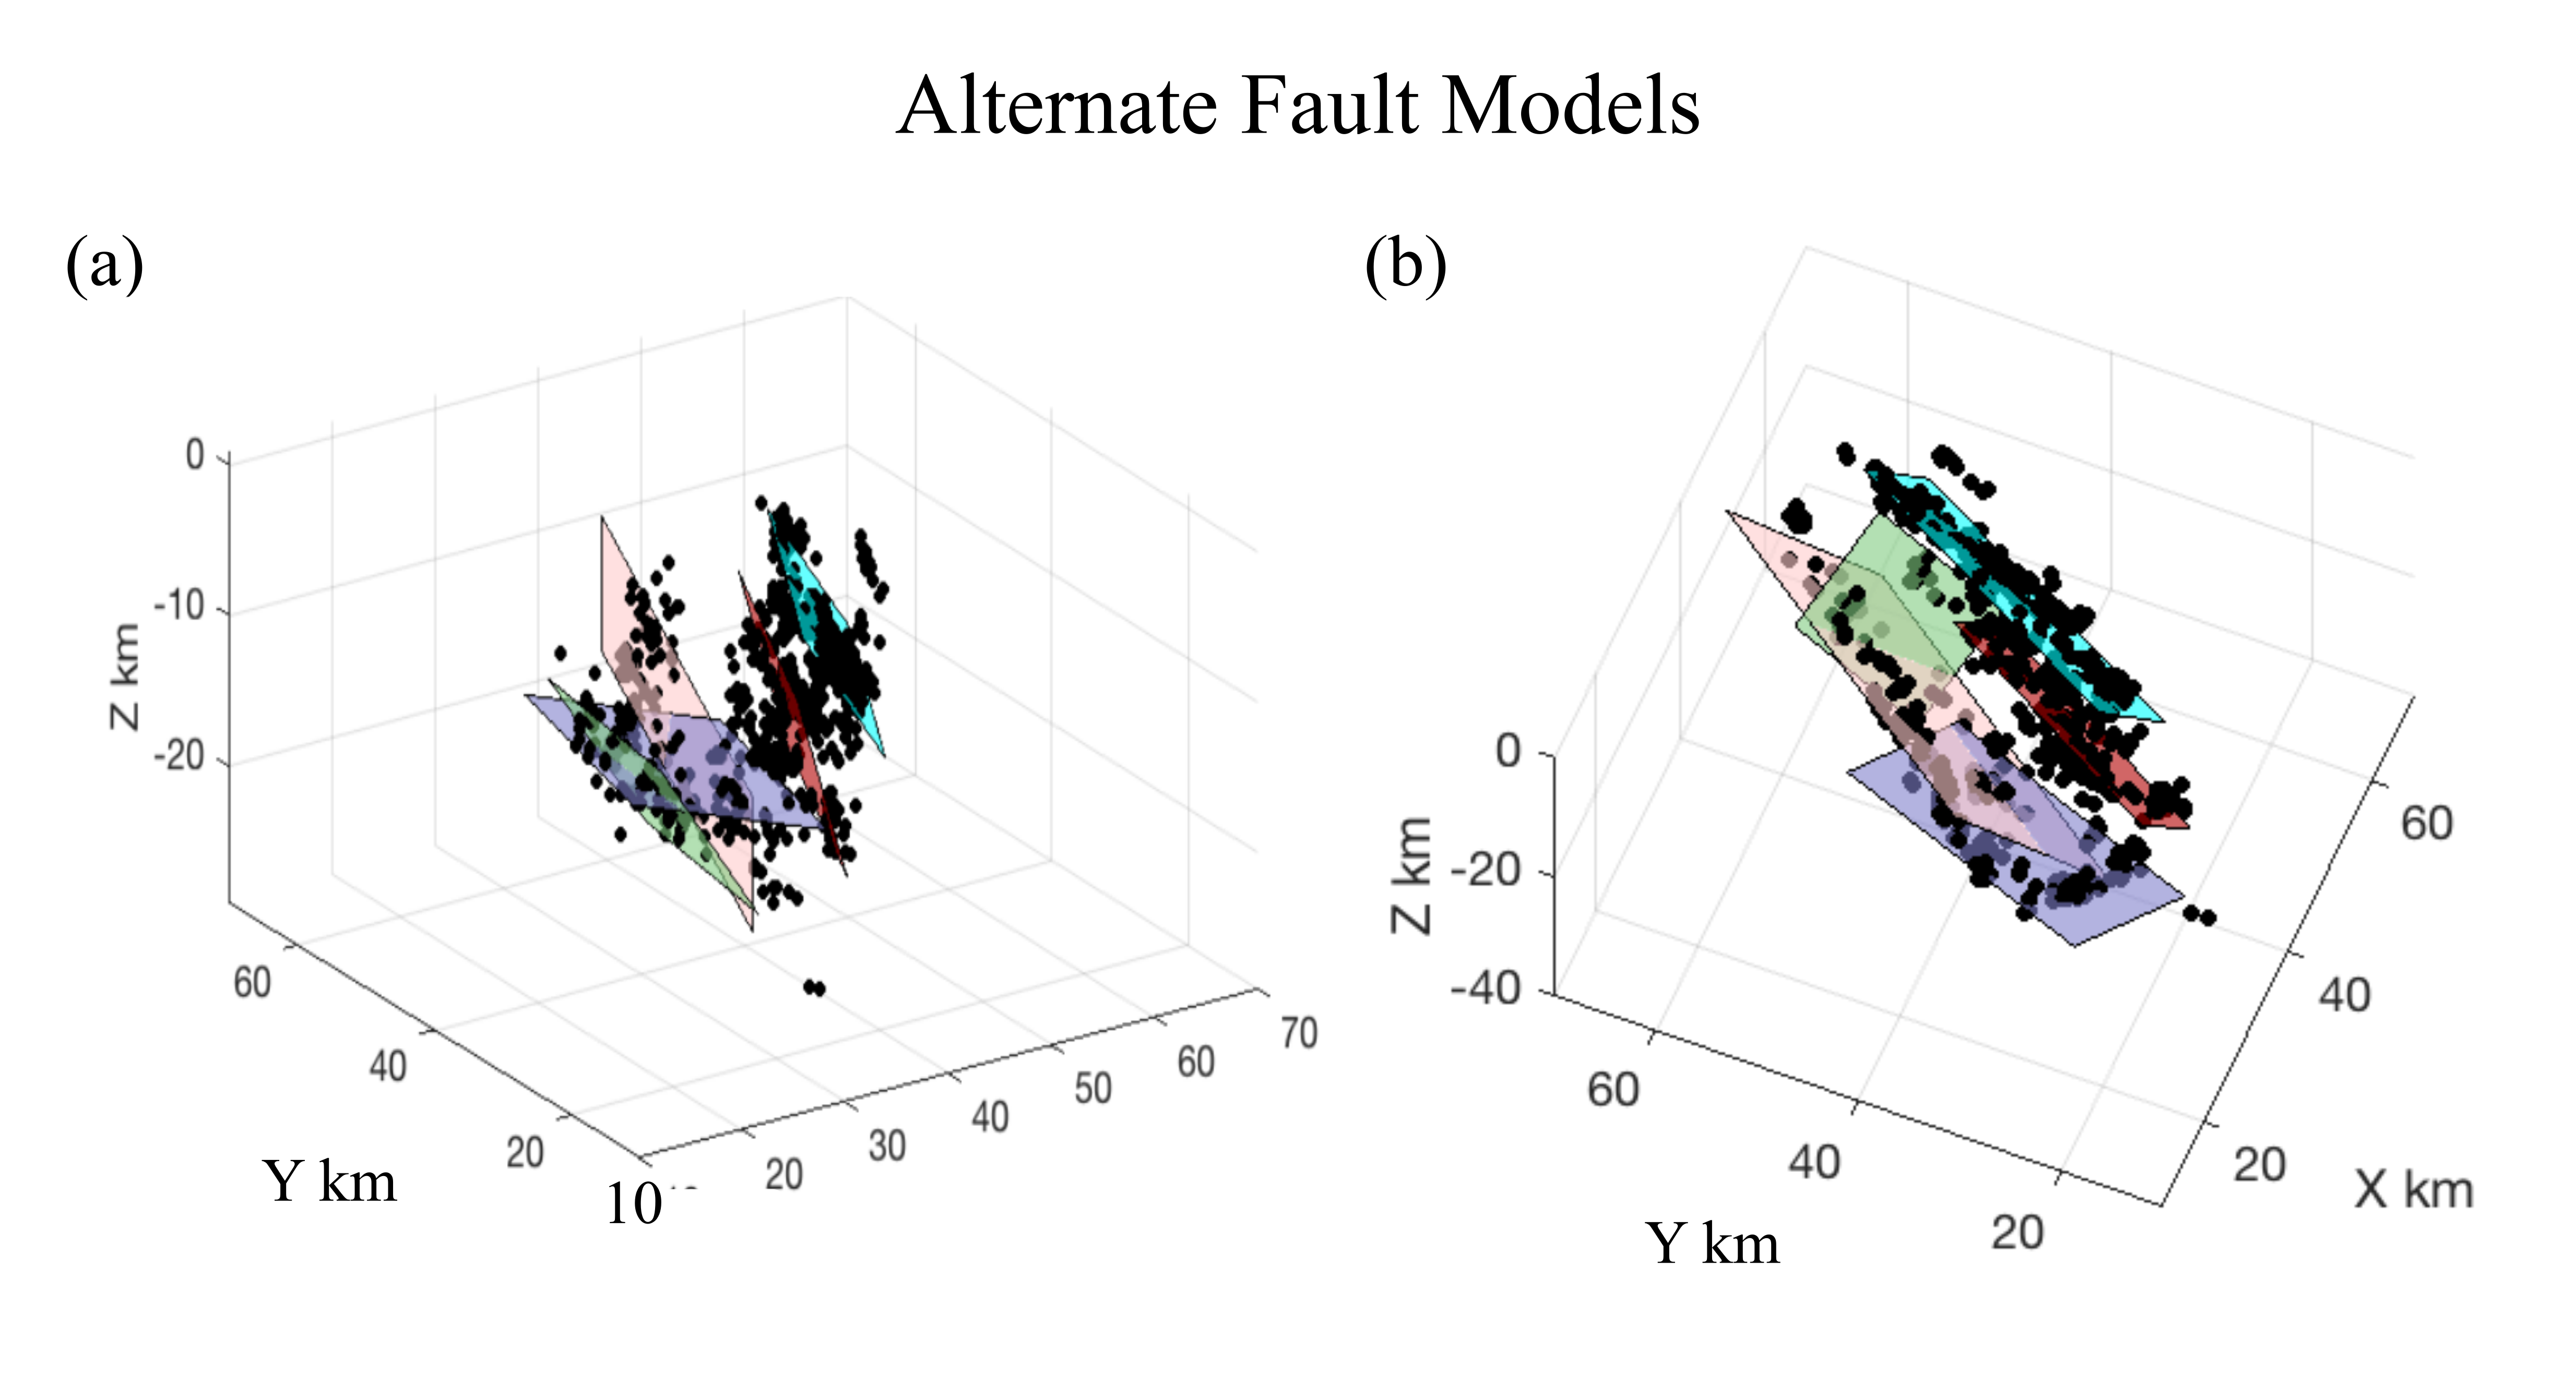
\includegraphics[width=25pc]{Figures/OADC_fig_alt_models.png}
\caption{Alternate fault models of OADC method.}
\label{figsix}
\end{figure}


   \begin{table}
    \caption{Fault geometry of the CSZ using OADC method.}
    \centering
    \begin{tabular}{ccccccccc}
    \hline
    Fault No &   & \multicolumn{2}{c}{Alternate Model 1$^{a}$} & &  \multicolumn{2}{c}{Alternate Model 2$^{a}$} & &  Possible mapped fault \\
     && Strike & Dip  & & Strike & Dip & & \\
    \hline
    1 & & 24.5$^\circ$ & 50.2$^\circ$ &   &     25.7$^\circ$ & 47.2$^\circ$&  &Charlevoix fault \\
    2 & & 177.6$^\circ$ & 12.0$^\circ$ & & 	5.8$^\circ$ & 22.6$^\circ$&  &Crater boundary  \\
    3 & & 24.2$^\circ$ & 71.4$^\circ$ & 	 &	32.3$^\circ$ & 50.7$^\circ$& & Saint-Laurent fault\\
    4 &  &5.7$^{\circ,b}$ & 50.3$^{\circ,b}$ &  &		116.3$^{\circ,c}$ & 72.47$^{\circ,c}$& &  \\
    5 &  &30.4$^\circ$ & 56.3$^\circ$ & 	 &	29.2$^\circ$ & 50.7$^\circ$&  &Gouffre Northwest fault\\
    \hline
     \multicolumn{9}{l}{$^{a}$ $\lambda_{3,max}$ for alternative models 1 and 2 are 1.59 and 1.53, respectively.}\\
    \multicolumn{9}{l}{$^{b}$ Possible continuation of the Gouffre Northwest fault to the southwest. $^{c}$ Spurious fault.}
    \end{tabular}
    \label{tableone}
    \end{table}


\section{Discussion}
In this section, we will discuss the unclustered and clustered hypocenters, and the limitations of the OADC from this study.

\subsection{Unclustered seismicity}
\textit{\textbf{The removal of the Unclustered seismicity decrease the fuzziness of earthquake distribution in the CSZ, thereby highlighting the rift faults (Figs. 2A and C).}} The unclustered earthquakes do not have inherent structure showing the rift faults, which suggests that they do not occurred on the major rift faults in the CSZ. The lack of inherent alignment validate the declustering method has not removing clustered hypocenters. Powell and Lamontagne (2017) also shows that the rift faults can not be traced inside the crater region. In this method removes the fuzziness of the seismicity within the crater and thus, the faults can be followed all the crater within the crater region. Thereby, helps to constrain the geometry of the rift faults (Fig. 2C).

\textit{\textbf{The unclustered seismicity in the crater region shows the geometry of the crater (Figs. 2B and D).}} The unclustered seismicity in the crater region is the background seismicity, and is mainly within the crater region. These background seismicity highlights the damaged region of the crater (the inner circle in Figure 1). \textit{Create a 3D map of the removed seismicity to highlight the geometry of the crater.}

\textbf{\textit{Figure of the background seismicity showing the inner circle.}}
 



\subsection{Clustered seismicity}
\textit{\textbf{The clustered seismicity show identifiable planes revealing the geometry of the three major rift faults in the CSZ (Fig. 3D).}} The first fault dips at an angle of 60$^\circ$ while the other two main rift faults dip at 44$^\circ$ and 43$^\circ$, respectively (Fig. 4D). We need to plot the clustered earthquakes on a geologic map to see the difference. And also plot some cross-sections. The results from this study also support Powell and Lamontagne (2017) that the alignment of the earthquakes on identifiable planes suggests that the earthquakes occurred on the rift faults instead of concentrating within the fault volume as suggested by previous authors (e.g. Baird et al. 2010, Auglin, Lamontagne, Rondot). These fault geometries match the work by Powell and Lamontagne (2017). The rift faults in the OADC supports that the South Shore fault do not play a role in the seismicity of the CSZ.

\textit{\textbf{In addition to the simple geometry of the rift faults, the seismicity reveals a more complicated geometry (Fig. 4D).}} \textit{\textbf{There is a change in the strike of the rift faults.}} Similar to what we see on the fault trace on Figure 1. Within the crater region, the faults are farther apart and somewhat converge in the northeastern part of the seismic zone. The middle and Charlevoix fault are closer outside the crater region. This is contrary to the simple fault geometry employed in Fadugba et al. (2010) with constant distance separation between the rift faults.

\textit{\textbf{And also reveals a change of dip in the first rift faults (Fig. 3D).}} in the form of three segments. Outside the crater, the first rift fault follow the first order strikes of the rift faults. Along strike variation in the dip of the rift faults (Fadugba et al., 2019). Within the crater region, the faults dips at 33.4$^\circ$ and 34.8$^\circ$.

\textit{\textbf{The seismicity follows the crater boundary (Fig. 3D).}} especially well in the northeastern part of the crater, and the shows that the seismicity also wrap around and beneath the crater. This seismicity highlights the geometry of the crater thereby constraining the depth of the crater. 


Lambda3 is better to solve fitting horizontal plane fit.
Show two figures showing fit with both lambda3 and global variance.


The shallower dip planes are in probably in response to the earthquakes wrapping around the crater region.




\subsection{Limitation of OADC}
\textit{\textbf{The results of OADC algorithm may change for every run}} because the results depend on the initially random seed planes within each cluster. Therefore, we may need to repeat the algorithm several time until the fault geometry is geologically feasible. 

\textit{\textbf{The surface projection of the fault planes from OADC may not coincide the fault trace}} on the geologic map. We need to find out how it changes.



\section{Conclusions}
The first fault dips at an angle of 60$^\circ$ while the other two main rift faults dip at 44$^\circ$ and 43$^\circ$, respectively. These fault geometries match the work by Powell and Lamontagne (2017). The rift faults show a more complicated geometry than the simple three-faults model in previous works, especially within the crater region. Within the crater region, the faults dips at 33.4$^\circ$ and 34.8$^\circ$. 




















%%%%%%%%%%%%%%
% Acronyms
\begin{acronyms}
 \acro{CSZ}
  Charlevoix Seismic Zone
 \acro{SH$_{\max}$}
  Maximum horizontal principal stress 
 \acro{OADC}
  Optimal Anisotropic Dynamic Clustering  
  \acro{ACLUD}
   Anisotropic Clustering of Location Uncertainty Distributions
  \acro{CDF}
  Cumulative Distribution Function
\end{acronyms}


%%%%%%%%%%%%%%
% Acknowledgments
\acknowledgments
This research was supported by Center for Earthquake Research and Information, University of Memphis.


%%%%%%%%%%%%%%
% Citation
%% Example \citet and \citep:
%  ...as shown by \citet{Boug10}, \citet{Buiz07}, \citet{Fra10},
%  \citet{Ghel00}, and \citet{Leit74}. 

%  ...as shown by \citep{Boug10}, \citep{Buiz07}, \citep{Fra10},
%  \citep{Ghel00, Leit74}. 

%  ...has been shown \citep [e.g.,][]{Boug10,Buiz07,Fra10}.

\bibliography{biblio}











%%%%%%%%%%%%%%%%%%%%%%%%%%%%%%%%%%%%%%%%%%%%%%%


%%

%  Numbered lines in equations:
%  To add line numbers to lines in equations,
%  \begin{linenomath*}
%  \begin{equation}
%  \end{equation}
%  \end{linenomath*}

%% Enter Figures and Tables near as possible to where they are first mentioned:
%
% DO NOT USE \psfrag or \subfigure commands.
%
% Figure captions go below the figure.
% Table titles go above tables;  other caption information
%  should be placed in last line of the table, using
% \multicolumn2l{$^a$ This is a table note.}
%
%----------------
% EXAMPLE FIGURE
%
% \begin{figure}[h]
% \centering
% when using pdflatex, use pdf file:
% \includegraphics[width=20pc]{figsamp.pdf}
%
% when using dvips, use .eps file:
% \includegraphics[width=20pc]{figsamp.eps}
%
% \caption{Short caption}
% \label{figone}
%  \end{figure}
%
% ---------------
% EXAMPLE TABLE
%
% \begin{table}
% \caption{Time of the Transition Between Phase 1 and Phase 2$^{a}$}
% \centering
% \begin{tabular}{l c}
% \hline
%  Run  & Time (min)  \\
% \hline
%   $l1$  & 260   \\
%   $l2$  & 300   \\
%   $l3$  & 340   \\
%   $h1$  & 270   \\
%   $h2$  & 250   \\
%   $h3$  & 380   \\
%   $r1$  & 370   \\
%   $r2$  & 390   \\
% \hline
% \multicolumn{2}{l}{$^{a}$Footnote text here.}
% \end{tabular}
% \end{table}

%% SIDEWAYS FIGURE and TABLE 
% AGU prefers the use of {sidewaystable} over {landscapetable} as it causes fewer problems.
%
% \begin{sidewaysfigure}
% \includegraphics[width=20pc]{figsamp}
% \caption{caption here}
% \label{newfig}
% \end{sidewaysfigure}
% 
%  \begin{sidewaystable}
%  \caption{Caption here}
% \label{tab:signif_gap_clos}
%  \begin{tabular}{ccc}
% one&two&three\\
% four&five&six
%  \end{tabular}
%  \end{sidewaystable}

%% If using numbered lines, please surround equations with \begin{linenomath*}...\end{linenomath*}
%\begin{linenomath*}
%\begin{equation}
%y|{f} \sim g(m, \sigma),
%\end{equation}
%\end{linenomath*}

%%% End of body of article

%%%%%%%%%%%%%%%%%%%%%%%%%%%%%%%%
%% Optional Appendix goes here
%
% The \appendix command resets counters and redefines section heads
%
% After typing \appendix
%
%\section{Here Is Appendix Title}
% will show
% A: Here Is Appendix Title
%
%\appendix
%\section{Here is a sample appendix}

%%%%%%%%%%%%%%%%%%%%%%%%%%%%%%%%%%%%%%%%%%%%%%%%%%%%%%%%%%%%%%%%
%
% Optional Glossary, Notation or Acronym section goes here:
%
%%%%%%%%%%%%%%  
% Glossary is only allowed in Reviews of Geophysics
%  \begin{glossary}
%  \term{Term}
%   Term Definition here
%  \term{Term}
%   Term Definition here
%  \term{Term}
%   Term Definition here
%  \end{glossary}

%
%%%%%%%%%%%%%%
% Acronyms
%\begin{acronyms}
% \acro{CSZ}
%  Charlevoix Seismic Zone
% \acro{SH$_{max}$}
%  Maximum horinzontal principal stress 
%\end{acronyms}

%
%%%%%%%%%%%%%%
% Notation 
%   \begin{notation}
%   \notation{$a+b$} Notation Definition here
%   \notation{$e=mc^2$} 
%   Equation in German-born physicist Albert Einstein's theory of special
%  relativity that showed that the increased relativistic mass ($m$) of a
%  body comes from the energy of motion of the body—that is, its kinetic
%  energy ($E$)—divided by the speed of light squared ($c^2$).
%   \end{notation}




%%%%%%%%%%%%%%%%%%%%%%%%%%%%%%%%%%%%%%%%%%%%%%%%%%%%%%%%%%%%%%%%
%
%  ACKNOWLEDGMENTS
%
% The acknowledgments must list:
%
% •	All funding sources related to this work from all authors
%
% •	Any real or perceived financial conflicts of interests for any
%	author
%
% •	Other affiliations for any author that may be perceived as
% 	having a conflict of interest with respect to the results of this
% 	paper.
%
% •	A statement that indicates to the reader where the data
% 	supporting the conclusions can be obtained (for example, in the
% 	references, tables, supporting information, and other databases).
%
% It is also the appropriate place to thank colleagues and other contributors. 
% AGU does not normally allow dedications.








%% ------------------------------------------------------------------------ %%
%% Citations

% Please use ONLY \citet and \citep for reference citations.
% DO NOT use other cite commands (e.g., \cite, \citeyear, \nocite, \citealp, etc.).


%% Example \citet and \citep:
%  ...as shown by \citet{Boug10}, \citet{Buiz07}, \citet{Fra10},
%  \citet{Ghel00}, and \citet{Leit74}. 

%  ...as shown by \citep{Boug10}, \citep{Buiz07}, \citep{Fra10},
%  \citep{Ghel00, Leit74}. 

%  ...has been shown \citep [e.g.,][]{Boug10,Buiz07,Fra10}.



%%  REFERENCE LIST AND TEXT CITATIONS
%
% Either type in your references using
%
% \begin{thebibliography}{}
% \bibitem[{\textit{Kobayashi et~al.}}(2003)]{R2013} Kobayashi, T.,
% Tran, A.~H., Nishijo, H., Ono, T., and Matsumoto, G.  (2003).
% Contribution of hippocampal place cell activity to learning and
% formation of goal-directed navigation in rats. \textit{Neuroscience}
% 117, 1025--1035.
%
% \bibitem{}
% Text
% \end{thebibliography}
%
%%%%%%%%%%%%%%%%%%%%%%%%%%%%%%%%%%%%%%%%%%%%%%%
% Or, to use BibTeX:
%
% Follow these steps
%
% 1. Type in \bibliography{<name of your .bib file>} 
%    Run LaTeX on your LaTeX file.
%
% 2. Run BiBTeX on your LaTeX file.
%
% 3. Open the new .bbl file containing the reference list and
%   copy all the contents into your LaTeX file here.
%
% 4. Run LaTeX on your new file which will produce the citations.
%
% AGU does not want a .bib or a .bbl file. Please copy in the contents of your .bbl file here.

%\bibliography{bibliography/biblio} 

%% After you run BibTeX, Copy in the contents of the .bbl file here:

\end{document}

%%%%%%%%%%%%%%%%%%%%%%%%%%%%%%%%%%%%%
%% Supporting Information
%% (Optional) See AGUSuppInfoSamp.tex/pdf for requirements 
%% for Supporting Information.
%%%%%%%%%%%%%%%%%%%%%%%%%%%%%%%%%%%%%



%%%%%%%%%%%%%%%%%%%%%%%%%%%%%%%%%%%%%%%%%%%%%%%%%%%%%%%%%%%%%%%

More Information and Advice:

%% ------------------------------------------------------------------------ %%
%
%  SECTION HEADS
%
%% ------------------------------------------------------------------------ %%

% Capitalize the first letter of each word (except for
% prepositions, conjunctions, and articles that are
% three or fewer letters).

% AGU follows standard outline style; therefore, there cannot be a section 1 without
% a section 2, or a section 2.3.1 without a section 2.3.2.
% Please make sure your section numbers are balanced.
% ---------------
% Level 1 head
%
% Use the \section{} command to identify level 1 heads;
% type the appropriate head wording between the curly
% brackets, as shown below.
%
%An example:
%\section{Level 1 Head: Introduction}
%
% ---------------
% Level 2 head
%
% Use the \subsection{} command to identify level 2 heads.
%An example:
%\subsection{Level 2 Head}
%
% ---------------
% Level 3 head
%
% Use the \subsubsection{} command to identify level 3 heads
%An example:
%\subsubsection{Level 3 Head}
%
%---------------
% Level 4 head
%
% Use the \subsubsubsection{} command to identify level 3 heads
% An example:
%\subsubsubsection{Level 4 Head} An example.
%
%% ------------------------------------------------------------------------ %%
%
%  IN-TEXT LISTS
%
%% ------------------------------------------------------------------------ %%
%
% Do not use bulleted lists; enumerated lists are okay.
% \begin{enumerate}
% \item
% \item
% \item
% \end{enumerate}
%
%% ------------------------------------------------------------------------ %%
%
%  EQUATIONS
%
%% ------------------------------------------------------------------------ %%

% Single-line equations are centered.
% Equation arrays will appear left-aligned.

Math coded inside display math mode \[ ...\]
 will not be numbered, e.g.,:
 \[ x^2=y^2 + z^2\]

 Math coded inside \begin{equation} and \end{equation} will
 be automatically numbered, e.g.,:
 \begin{equation}
 x^2=y^2 + z^2
 \end{equation}


% To create multiline equations, use the
% \begin{eqnarray} and \end{eqnarray} environment
% as demonstrated below.
\begin{eqnarray}
  x_{1} & = & (x - x_{0}) \cos \Theta \nonumber \\
        && + (y - y_{0}) \sin \Theta  \nonumber \\
  y_{1} & = & -(x - x_{0}) \sin \Theta \nonumber \\
        && + (y - y_{0}) \cos \Theta.
\end{eqnarray}

%If you don't want an equation number, use the star form:
%\begin{eqnarray*}...\end{eqnarray*}

% Break each line at a sign of operation
% (+, -, etc.) if possible, with the sign of operation
% on the new line.

% Indent second and subsequent lines to align with
% the first character following the equal sign on the
% first line.

% Use an \hspace{} command to insert horizontal space
% into your equation if necessary. Place an appropriate
% unit of measure between the curly braces, e.g.
% \hspace{1in}; you may have to experiment to achieve
% the correct amount of space.


%% ------------------------------------------------------------------------ %%
%
%  EQUATION NUMBERING: COUNTER
%
%% ------------------------------------------------------------------------ %%

% You may change equation numbering by resetting
% the equation counter or by explicitly numbering
% an equation.

% To explicitly number an equation, type \eqnum{}
% (with the desired number between the brackets)
% after the \begin{equation} or \begin{eqnarray}
% command.  The \eqnum{} command will affect only
% the equation it appears with; LaTeX will number
% any equations appearing later in the manuscript
% according to the equation counter.
%

% If you have a multiline equation that needs only
% one equation number, use a \nonumber command in
% front of the double backslashes (\\) as shown in
% the multiline equation above.

% If you are using line numbers, remember to surround
% equations with \begin{linenomath*}...\end{linenomath*}

%  To add line numbers to lines in equations:
%  \begin{linenomath*}
%  \begin{equation}
%  \end{equation}
%  \end{linenomath*}


%%%%%%%%%%%%%%%%%%%%%%%%%%%%%%%%%%%%%%%%%%%%%%%
\section{Model Setup}
We create numerical models 

\subsection{Model geometry}
Our models are composed of three units, crust, crater and rift faults, reflecting a simplification of the geology of the region (Fig. \ref{figtwo}A). The crust is a 220 $\times$ 220 $\times$ 40 km box with the crater cut out. 

\subsection{Initial and boundary conditions}
\label{Initial_and_boundary_conditions}
Initial stresses are assumed to be lithostatic. %Including gravity has the effect of increasing normal stress and decreasing the amount of slip on the rift faults with depth. 

\subsection{Control Parameters}
%\subsection{Parameters to control}
We create a series of models in which the following parameters are varied: dips of the rift faults, friction coefficients, % and cohesion of the faults, 
crater-crust elastic moduli ratios, and the velocity models. Two fault geometries for the CSZ are considered. One model has a dip angle of 70$^\circ$SE for all three rift faults~\citep{Baird_2010}. The other assumes that the three faults have dip angles of 65$^\circ$SE, 40$^\circ$SE and 
%
%\begin{comment}
\begin{table}
\caption{List of numerical models}%\note[EC]{Please check the ranges of mu and C.}}
\centering
\begin{tabular}{llccccc}
\hline
Model & Velocity Model & Dip of Rift Faults & Moduli ratio & $\mu$ & C  \\
\hline
SNFR25  & Saguenay Region$^{1}$ & No faults & 0.25 & 0.3 & 0 \\
SD70R25  &  & $70^\circ-70^\circ-70^\circ$  & 0.25 & 0.3 & 0 \\
SD70R25V  &  & $70^\circ-70^\circ-70^\circ$  & 0.25 & 0.1-0.6 & 0 \\
%SD70R25M1 &  & $70^\circ-70^\circ-70^\circ$  & 0.25 & 0.1 & 0 \\
SD65R25  &  & $65^\circ-40^\circ-40^\circ$  & 0.25 & 0.3 & 0\\
SD70R50  &  & $70^\circ-70^\circ-70^\circ$  & 0.5 & 0.3 & 0 \\
SD70R100   &  & $70^\circ-70^\circ-70^\circ$  & 1.0 & 0.3 & 0 \\
LD70R25 & 1-D Model$^{2}$ & $70^\circ-70^\circ-70^\circ$ & 0.25 & 0.3  & 0 \\
TD70 & Tomography$^{3}$ & $70^\circ-70^\circ-70^\circ$ & - & 0.3 & 0 \\
\hline
\multicolumn{6}{l}{$^{1}$\citet{Somerville1990}. $^{2}$\citet{lamontagne1999}. $^{3}$\citet{Powell_2017}.}
\end{tabular}
\label{tableone}
\end{table}
%\end{comment}


% ###################################################################################################################

\section{Results}

%\begin{comment}
\subsection{Reference Model (SNFR25)} \label{Ref_Model}
%The model SD70R25 has three rift faults, all of which have a dip of 70$^{\circ}$SE. We first describe the stress field in SNFR25 (no-fault version of SD70R25 model) and SD70R25 models in terms of the $\sigma_D$ and $\phi_{\max}$ at depths 5, 10, 15, 20 and 25 km. We then compare the SD70R25 model with the fault-free SNFR25 model in terms of the $\Delta\sigma_D^{\prime}$ and $\Delta \phi_{\max}$ because the effects of faults on stress distributions are best highlighted by the differences between them. 
The effects of the weaker crater are dominant in SNFR25. $\sigma_D$ is smaller by 100s MPa in the crater region relative to the surrounding crustal rock as shown by 5 and 10-km depth sections (Fig. \ref{fig:SNFR25_ref}A). The absolute value of $\sigma_D$ is greater (i.e. is more negative) in the direction perpendicular to the applied loading than in the parallel direction. At depths below the crater (i.e., depths $\ge$ 15 km), $\sigma_D$ is more negative 
%greater 
% #############################################################
\subsection{Effects of rift faults and their dip}
\subsubsection{SD70R25}
Magnitudes of $\sigma_{D}$ in SD70R25 are smaller in the crater than in the surrounding crust, as in the reference model, but also significantly modified by abrupt changes in the vicinity of the rift faults (Fig. \ref{fig:SD70R25}A). $\sigma_{D}$ at a distance greater than 50 km from the center of the crater is similar to that of the reference model at each depth. 
%

% #############################################################

\subsubsection{SD65R25}

\subsection{Effects of the weakness of the damaged crater zone}
%Stress fields associated with various strengths of the damaged crater region are described in terms of $\sigma_D$ and $\phi_{\max}$. 
Two models with the rift faults dipping at 70$^{\circ}$ are constructed such that the ratio of elastic moduli of the crater to that of the surrounding crust are 0.5 (SD70R50) and 1.0 (SD70R100), respectively. 
%These models are compared with the model SD70R25, for which the crater-to-crust ratio of elastic moduli is 0.25.

\subsubsection{SD70R50}
While the effects of the crater and rift faults are still clear and consistent, SD70R50 values of $\Delta \sigma_{D}^{\prime}$ are mostly negative with some exceptions at 10 km depth amounting to about a 10 \% increased stress (Fig. \ref{fig:eff_of_moduli_ratio}A).
%

% #############################################################
\subsubsection{SD70R100}
%SD70R100 shows only the effects of the rift faults since the crater and the crust have the same elastic moduli (Fig. \ref{fig:eff_of_moduli_ratio}B). $\Delta\sigma_D^{\prime}$ and $\phi_{\max}$ %are significantly 
%exhibit only the effects of the rift faults. 

$\Delta\sigma_D^{\prime}$ and $\phi_{\max}$ only exhibit the effects of the rift faults since the crater and the crust have the same elastic moduli in model SD70R100 (Fig. \ref{fig:eff_of_moduli_ratio}B).







\begin{figure}[h]
\centering
\includegraphics[width=20pc]{Figures/Map_of_CSV_now3.png} %_lowq
\caption{Topography and seismicity of the Charlevoix Seismic Zone (CSZ) as well as the locations of the impact crater (outer cyan circle) and the more damaged inner crater (inner cyan circle). Small circles are the relocated epicenters \citep{Powell_2017} and their colors represent the focal depths. The focal mechanisms are for the earthquakes used by \citet{Mazzotti_2010} for the stress inversion. Large circles labeled as NW and SE show orientations of SH$_{\max}$ from the stress inversion of focal mechanism (SH$_S$) and from borehole breakout measurements (SH$_B$) for the earthquake clusters northwest and southeast of the crater center. Solid black lines mark the rift faults known in the region: GNF, Gouffre Northwest Fault; SLF, Saint-Laurent fault; CHF, Charlevoix Fault; and SSF, South Shore Fault \citep{Rondot_1971,lamontagne1999}. The inset shows the location of the CSZ in eastern Canada. Earthquake epicenters from the National Resources Canada catalog for the years 1988-2011.}
\label{figone}
\end{figure}
%\end{comment}


\begin{table}
\caption{List of numerical models}%\note[EC]{Please check the ranges of mu and C.}}
\centering
\begin{tabular}{llccccc}
\hline
Model & Velocity Model & Dip of Rift Faults & Moduli ratio & $\mu$ & C  \\
\hline
SNFR25  & Saguenay Region$^{1}$ & No faults & 0.25 & 0.3 & 0 \\
SD70R25  &  & $70^\circ-70^\circ-70^\circ$  & 0.25 & 0.3 & 0 \\
SD70R25V  &  & $70^\circ-70^\circ-70^\circ$  & 0.25 & 0.1-0.6 & 0 \\
%SD70R25M1 &  & $70^\circ-70^\circ-70^\circ$  & 0.25 & 0.1 & 0 \\
SD65R25  &  & $65^\circ-40^\circ-40^\circ$  & 0.25 & 0.3 & 0\\
SD70R50  &  & $70^\circ-70^\circ-70^\circ$  & 0.5 & 0.3 & 0 \\
SD70R100   &  & $70^\circ-70^\circ-70^\circ$  & 1.0 & 0.3 & 0 \\
LD70R25 & 1-D Model$^{2}$ & $70^\circ-70^\circ-70^\circ$ & 0.25 & 0.3  & 0 \\
TD70 & Tomography$^{3}$ & $70^\circ-70^\circ-70^\circ$ & - & 0.3 & 0 \\
\hline
\multicolumn{6}{l}{$^{1}$\citet{Somerville1990}. $^{2}$\citet{lamontagne1999}. $^{3}$\citet{Powell_2017}.}
\end{tabular}
\label{tableone}
\end{table}









\section{Discussions}

\subsection{Earthquake distribution}
Our models suggest that having both the rift faults and the impact crater is not only sufficient but also necessary for explaining the distribution of earthquakes in the CSZ.
% in terms of both magnitudes and frequencies.

\subsection{Spatial variations of SH$_{\max}$ orientation}
%Our study explains the stress rotations in the CSZ relative to the regional stress orientation, and the stress rotation between NW and SE earthquake clusters. Our model also explains the other of stress rotations with respect to the %This observation 
suggests that the presence of the rift faults and the relative angles of their strikes with respect to the regional orientation of SH$_{\max}$ alone can result in stress rotations ~\citep[e.g.,][]{Zoback_1992}. However, the combined effect of the impact crater with up to a quarter of the elastic moduli of the surrounding crust, and the rift faults are required in the CSZ to explain the observed clockwise rotations of the $\phi_{\max}$ in the SE cluster of earthquakes relative to the NW cluster, as well as in the entire CSZ relative to the direction of regional tectonic loading.
% -----------------------------------------------------------------------

